\documentclass[]{article}
\usepackage{amsfonts}
\usepackage{pgfplots}
\usetikzlibrary{math}
\usetikzlibrary{perspective}
\usepackage{amsmath}
\usepackage{lmodern}
\usepackage[T1]{fontenc}
\usepackage{setspace}
%\usepackage{fullpage}
%\pgfplotsset{compat=1.15}

\renewcommand{\div}{\mathrm {div}}
\DeclareMathOperator{\curl}{curl}
\DeclareMathOperator{\ran}{ran}

\definecolor{newcolor}{RGB}{.8,.349,.1}
\definecolor{lightgray}{RGB}{200,200,200}
%%%%%emph colors
\definecolor{emph1}{RGB}{0,102,153}
\definecolor{emph2}{RGB}{200,90,20}
\definecolor{emph3}{RGB}{100,30,153}
\definecolor{emph4}{RGB}{0,100,0}
\definecolor{emph5}{RGB}{0,100,200}
\definecolor{emph6}{RGB}{100,0,0}

%for image output uncomment the following two lines and the pgf plot paragraph and compile with --shell-escape
\usepgfplotslibrary{external}
\tikzexternalize[prefix=images/]


\begin{document}


%%%%macros for drawing dofs
\newcommand{\trig}{%
  \draw[thick,gray](0,0)--++(4,0)--++(-4,4)--++(0,-4);
    \draw(0+2,0)--(0+4/3,0+4/3)--(0,0+2);
    \draw(0+2,0+2)--(0+4/3,0+4/3);
    }
\newcommand{\trigmethod}{%
  %\filldraw[fill=orange!30,thick,draw=gray](0,0)--++(4,0)--++(-4,4)--++(0,-4);
  \draw[thick](0,0)--++(4,0)--++(-4,4)--++(0,-4);
    %\filldraw[fill=orange!30](0+2,0)--(0+4/3,0+4/3)--(0,0+2);
    %\filldraw[fill=orange!30](0+2,0+2)--(0+4/3,0+4/3);
    \draw(0+2,0)--(0+4/3,0+4/3)--(0,0+2);
    \draw(0+2,0+2)--(0+4/3,0+4/3);
    \fill[fill=orange!30](0,0)--(0+2,0)--(0+4/3,0+4/3)--(0,0+2)--(0,0);
    }
\newcommand\dof[4][]{%
  \node[#1] at (2*#2-4/6*#2*#3,2*#3-4/6*#2*#3){};
  \node[] at (2*#2-4/6*#2*#3-0.1,2*#3-4/6*#2*#3-0.3){\small #4};
  %\node[#1] at (2*#3-4/6*#2*#3,4-2*#2+4/6*#2*#3-2*#3+4/6*#2*#3){};
  %\node[#1] at (4-2*#2+4/6*#2*#3-2*#3+4/6*#2*#3,2*#2-4/6*#2*#3){};
}
\newcommand\dofprimal[4][]{%
  \node[#1] at (2*#2-4/6*#2*#3,2*#3-4/6*#2*#3){};
  \node[] at (2*#2-4/6*#2*#3-0.1,2*#3-4/6*#2*#3-0.3){\small #4};
  \node[#1] at (2*#3-4/6*#2*#3,4-2*#2+4/6*#2*#3-2*#3+4/6*#2*#3){};
  \node[#1] at (4-2*#2+4/6*#2*#3-2*#3+4/6*#2*#3,2*#2-4/6*#2*#3){};
}
\newcommand\innerdofprimal[2]{
  \dofprimal[circle,thick,draw=blue]{#1}{#2}{}
}
\newcommand\innerdof[2]{
  \dof[circle,thick,draw=blue]{#1}{#2}{}
}
\newcommand\innervdof[2]{
  \dof[circle,thick,draw=teal]{#1}{#2}{}
}
\newcommand\graydof[2]{
  \dof[circle,thick,fill=gray]{#1}{#2}{}
}
\newcommand\graydofpimal[2]{
  \dofprimal[circle,thick,fill=gray]{#1}{#2}{}
}
\newcommand\facedof[2]{
  \dof[circle,fill=purple]{#1}{#2}{}
}
\newcommand\facedofprimal[2]{
  \dofprimal[circle,fill=purple]{#1}{#2}{}
}
\newcommand\facedoflabel[3]{
  \dof[circle,fill=purple]{#1}{#2}{#3}
}
\newcommand\edgedof[2]{
  \dof[circle,fill=blue]{#1}{#2}{}
}
\newcommand\edgedofprimal[2]{
  \dofprimal[circle,fill=blue]{#1}{#2}{}
}
\newcommand\edgedoflabel[3]{
  \dof[circle,fill=blue]{#1}{#2}{#3}
}
\newcommand\vertexdof[2]{
  \dof[circle,fill=teal]{#1}{#2}{}
}
\newcommand\vertexdofprimal[2]{
  \dofprimal[circle,fill=teal]{#1}{#2}{}
}
\newcommand\vertexdoflabel[3]{
  \dof[circle,fill=teal]{#1}{#2}{#3}
}
\newcommand\arrowdof[6][]{
  \begin{scope}[]
    \draw[#1,very thick,-latex] (2*#2-4/6*#2*#3,2*#3-4/6*#2*#3)--node {#6}                 (2*#4-4/6*#4*#5,2*#5-4/6*#4*#5);
  %\draw[#1,very thick,-latex] (2*#3-4/6*#2*#3,4-2*#2+4/6*#2*#3-2*#3+4/6*#2*#3)--(2*#5-4/6*#4*#5,4-2*#4+4/6*#4*#5-2*#5+4/6*#4*#5);
  %\draw[#1,very thick,-latex] (4-2*#2+4/6*#2*#3-2*#3+4/6*#2*#3,2*#2-4/6*#2*#3)--(4-2*#4+4/6*#4*#5-2*#5+4/6*#4*#5,2*#4-4/6*#4*#5);
  \end{scope}
}
\newcommand\arrowdofprimal[6][]{
  \begin{scope}[]
    \draw[#1,very thick,-latex] (2*#2-4/6*#2*#3,2*#3-4/6*#2*#3)--node {#6}                 (2*#4-4/6*#4*#5,2*#5-4/6*#4*#5);
  \draw[#1,very thick,-latex] (2*#3-4/6*#2*#3,4-2*#2+4/6*#2*#3-2*#3+4/6*#2*#3)--(2*#5-4/6*#4*#5,4-2*#4+4/6*#4*#5-2*#5+4/6*#4*#5);
  \draw[#1,very thick,-latex] (4-2*#2+4/6*#2*#3-2*#3+4/6*#2*#3,2*#2-4/6*#2*#3)--(4-2*#4+4/6*#4*#5-2*#5+4/6*#4*#5,2*#4-4/6*#4*#5);
  \end{scope}
}
\newcommand\facearrowdof[4]{
  \arrowdof[purple]{#1}{#2}{#3}{#4}{}
}
\newcommand\edgearrowdof[4]{
  \arrowdof[blue]{#1}{#2}{#3}{#4}{}
}
\newcommand\innerarrowdof[4]{
  \arrowdof[blue,dotted]{#1}{#2}{#3}{#4}{}
}

\newcommand\facearrowdofprimal[4]{
  \arrowdofprimal[purple]{#1}{#2}{#3}{#4}{}
}
\newcommand\edgearrowdofprimal[4]{
  \arrowdofprimal[blue]{#1}{#2}{#3}{#4}{}
}
\newcommand\innerarrowdofprimal[4]{
  \arrowdofprimal[blue,dotted]{#1}{#2}{#3}{#4}{}
}

\tikzsetnextfilename{ring_resonator_geo}
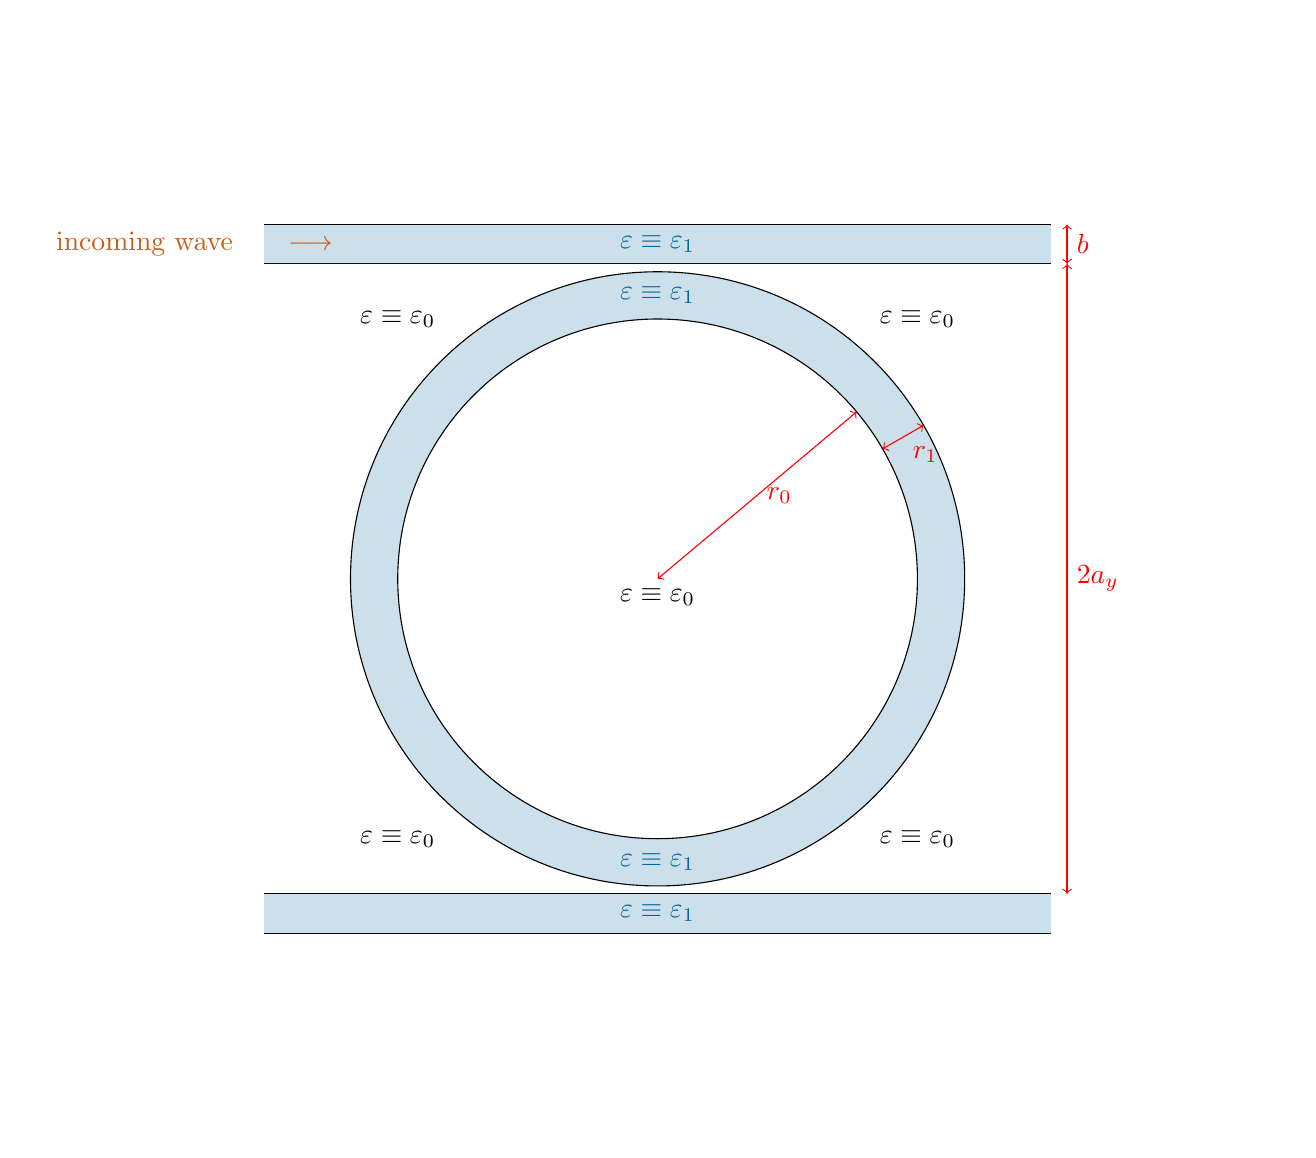
\begin{tikzpicture}
  \def\a{4};  
  \def\b{0.5};  
  \def\c{0.2};  
  \def\p{1};  
  \def\r{3.9};  
  \def\rr{3.3};  
  \def\bgx{-8};
  \def\bgxx{8};
  \def\bgy{-7}
  \def\bgyy{7}
  \fill[opacity=0.] (\bgx,\bgy)rectangle(\bgxx,\bgyy);
  %\draw[] (-\a,-\a-\b-\c)--++(2*\a,0)--++(0,2*\a+2*\b+2*\c)--++(-2*\a,0)--++(0,-2*\a-2*\b-2*\c);
  %\draw[] (-\a-\p,\a)--++(2*\a+2*\p,0);
  \draw[] (-\a-\p,\a)--++(2*\a+2*\p,0);
  \draw[] (-\a-\p,\a+\b)--++(2*\a+2*\p,0);
  %\draw[] (-\a-\p,\a+\b+\c)--++(2*\a+2*\p,0);
  \draw[] (-\a-\p,-\a)--++(2*\a+2*\p,0);
  \draw[] (-\a-\p,-\a-\b)--++(2*\a+2*\p,0);
  %\draw[] (-\a-\p,-\a-\b-\c)--++(2*\a+2*\p,0);
  %\draw[] (-\a,-\a-\b-\c-\p)--++(-\p,\p)--++(0,2*\a+2*\b+2*\c)--++(\p,\p);
  %\draw[] (\a,-\a-\b-\c-\p)--++(\p,\p)--++(0,2*\a+2*\b+2*\c)--++(-\p,\p);
  %\fill[opacity=0.2] (\a,-\a-\b-\c-\p)--++(\p,\p)--++(0,2*\a+2*\b+2*\c)--++(-\p,\p);
  %\fill[opacity=0.2] (-\a,-\a-\b-\c-\p)--++(-\p,\p)--++(0,2*\a+2*\b+2*\c)--++(\p,\p);
  %\fill[opacity=0.2] (-\a,-\a-\b-\c-\p)--++(0,\p)--++(2*\a,0)--++(0,-\p);
  %\fill[opacity=0.2] (-\a,\a+\b+\c)--++(0,\p)--++(2*\a,0)--++(0,-\p);
  \fill[emph1,opacity=0.2] (-\a-\p,\a)--++(0,\b)--++(2*\a+2*\p,0)--++(0,-\b);
  \fill[emph1,opacity=0.2] (-\a-\p,-\a-\b)--++(0,\b)--++(2*\a+2*\p,0)--++(0,-\b);
  \fill[emph1,opacity=0.2,even odd rule] (0,0) circle (\r) (0,0) circle (\rr);
  \draw (0,0) circle (\r);
  \draw (0,0) circle (\rr);
  \node[left,emph2] at (-\a,\a+0.5*\b){incoming wave\qquad $\longrightarrow$};
  \node[emph1] at (0,\a+\b/2) {$\varepsilon\equiv\varepsilon_1$};
  \node[emph1] at (0,-\a-\b/2) {$\varepsilon\equiv\varepsilon_1$};
  \node[emph1] at (0,\r/2+\rr/2) {$\varepsilon\equiv\varepsilon_1$};
  \node[emph1] at (0,-\r/2-\rr/2) {$\varepsilon\equiv\varepsilon_1$};
  \node[below] at (0,0) {$\varepsilon\equiv\varepsilon_0$};
  \node[] at (\rr,\rr) {$\varepsilon\equiv\varepsilon_0$};
  \node[] at (-\rr,-\rr) {$\varepsilon\equiv\varepsilon_0$};
  \node[] at (-\rr,\rr) {$\varepsilon\equiv\varepsilon_0$};
  \node[] at (\rr,-\rr) {$\varepsilon\equiv\varepsilon_0$};
  %measurements
  %\draw[<->, red] (\a+\p+\c,\a+\b+\c+\p)--node[right]{$p$}++(0,-\p);
  %\draw[<->, red] (\a+\p+\c,\a+\b+\c)--node[right]{$c$}++(0,-\c);
  \draw[<->, red] (\a+\p+\c,\a+\b)--node[right]{$b$}++(0,-\b);
  \draw[<->, red] (\a+\p+\c,\a)--node[right]{$2a_y$}++(0,-\a-\a);
  %\draw[<->, red] (-\a,\a+\b+\c+\p+\c)--node[above]{$2a_x$}++(\a+\a,0);
  \draw[<->, red] (0,0)--node[right]{$r_0$}++(40:\rr);
  \draw[<->, red] (30:\rr)--node[below right]{$r_1$}(30:\r);
\end{tikzpicture}

\tikzsetnextfilename{ring_resonator_geo_pml}
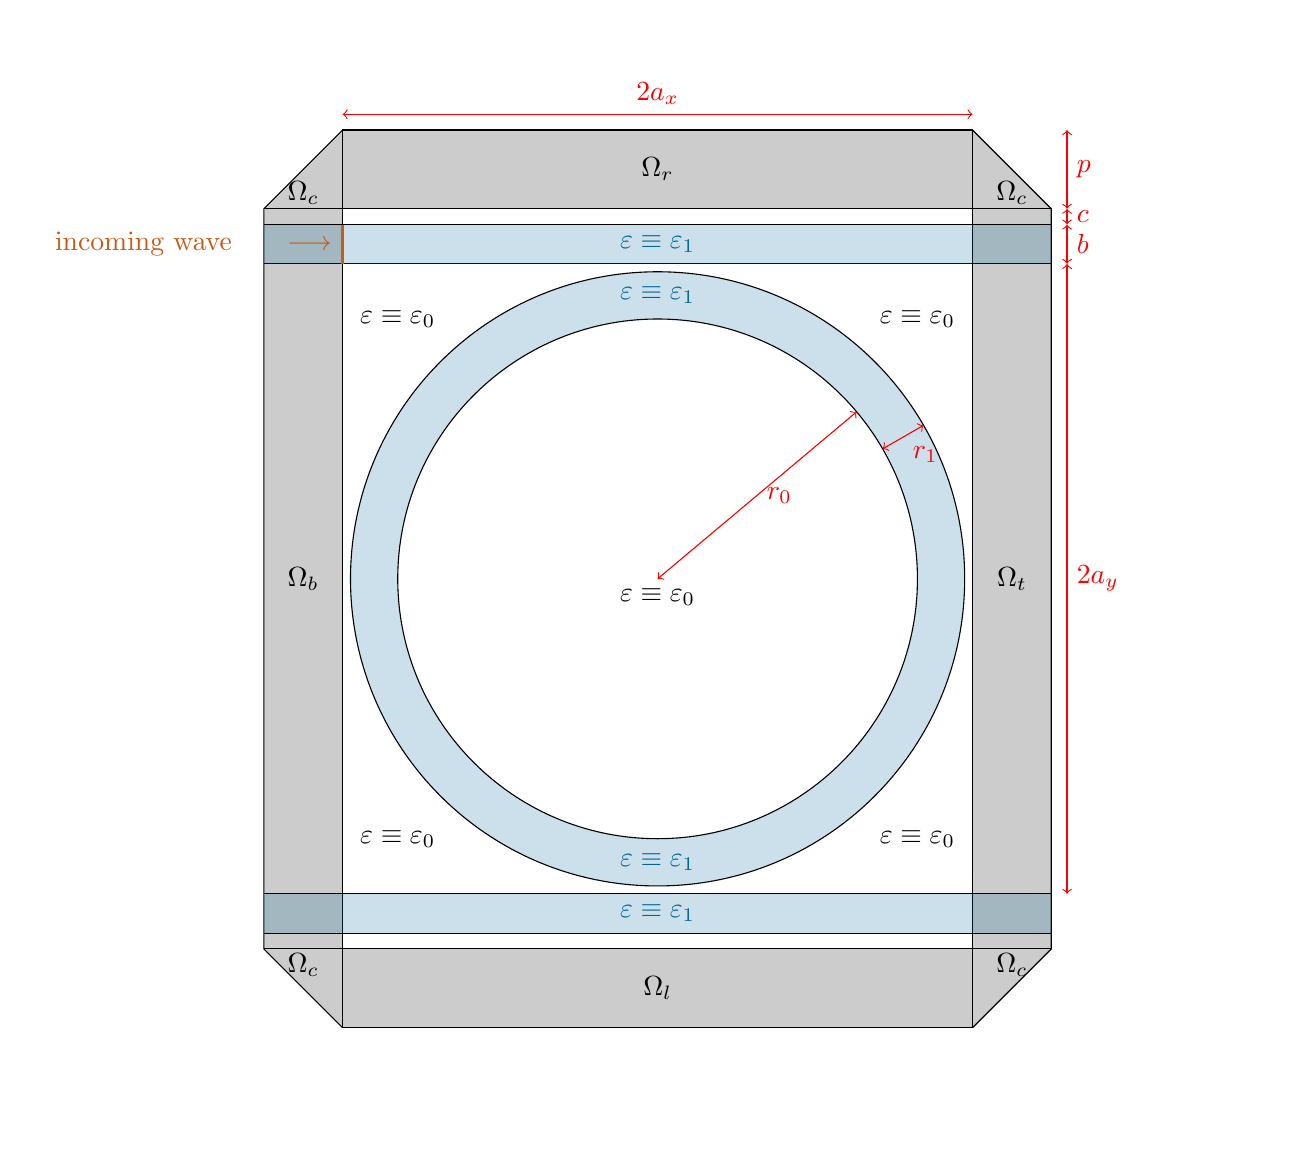
\begin{tikzpicture}
  \def\a{4};  
  \def\b{0.5};  
  \def\c{0.2};  
  \def\p{1};  
  \def\r{3.9};  
  \def\rr{3.3};  
  \def\bgx{-8};
  \def\bgxx{8};
  \def\bgy{-7}
  \def\bgyy{7}
  \fill[opacity=0.] (\bgx,\bgy)rectangle(\bgxx,\bgyy);
  \draw[] (-\a,-\a-\b-\c-\p)--++(2*\a,0)--++(0,2*\a+2*\b+2*\c+2*\p)--++(-2*\a,0)--++(0,-2*\a-2*\b-2*\c-2*\p);
  \draw[] (-\a-\p,\a)--++(2*\a+2*\p,0);
  \draw[] (-\a-\p,\a)--++(2*\a+2*\p,0);
  \draw[] (-\a-\p,\a+\b)--++(2*\a+2*\p,0);
  \draw[] (-\a-\p,\a+\b+\c)--++(2*\a+2*\p,0);
  \draw[] (-\a-\p,-\a)--++(2*\a+2*\p,0);
  \draw[] (-\a-\p,-\a-\b)--++(2*\a+2*\p,0);
  \draw[] (-\a-\p,-\a-\b-\c)--++(2*\a+2*\p,0);
  \draw[] (-\a,-\a-\b-\c-\p)--++(-\p,\p)--++(0,2*\a+2*\b+2*\c)--++(\p,\p);
  \draw[] (\a,-\a-\b-\c-\p)--++(\p,\p)--++(0,2*\a+2*\b+2*\c)--++(-\p,\p);
  \fill[opacity=0.2] (\a,-\a-\b-\c-\p)--++(\p,\p)--++(0,2*\a+2*\b+2*\c)--++(-\p,\p);
  \fill[opacity=0.2] (-\a,-\a-\b-\c-\p)--++(-\p,\p)--++(0,2*\a+2*\b+2*\c)--++(\p,\p);
  \fill[opacity=0.2] (-\a,-\a-\b-\c-\p)--++(0,\p)--++(2*\a,0)--++(0,-\p);
  \fill[opacity=0.2] (-\a,\a+\b+\c)--++(0,\p)--++(2*\a,0)--++(0,-\p);
  \fill[emph1,opacity=0.2] (-\a-\p,\a)--++(0,\b)--++(2*\a+2*\p,0)--++(0,-\b);
  \fill[emph1,opacity=0.2] (-\a-\p,-\a-\b)--++(0,\b)--++(2*\a+2*\p,0)--++(0,-\b);
  \fill[emph1,opacity=0.2,even odd rule] (0,0) circle (\r) (0,0) circle (\rr);
  \draw (0,0) circle (\r);
  \draw (0,0) circle (\rr);
  \draw[very thick, emph2] (-\a,\a)--node[left]{incoming wave\qquad $\longrightarrow$}++(0,\b);
  \node at (0,\a+\b+\c+\p/2) {$\Omega_r$};
  \node at (0,-\a-\b-\c-\p/2) {$\Omega_l$};
  \node at (\a+\b+\c-\p/5,0) {$\Omega_t$};
  \node at (-\a-\b-\c+\p/5,0) {$\Omega_b$};
  \node at (-\a-\b-\c+\p/5,-\a-\b-\c-\p/5) {$\Omega_c$};
  \node at (+\a+\b+\c-\p/5,-\a-\b-\c-\p/5) {$\Omega_c$};
  \node at (-\a-\b-\c+\p/5,\a+\b+\c+\p/5) {$\Omega_c$};
  \node at (+\a+\b+\c-\p/5,\a+\b+\c+\p/5) {$\Omega_c$};
  \node[emph1] at (0,\a+\b/2) {$\varepsilon\equiv\varepsilon_1$};
  \node[emph1] at (0,-\a-\b/2) {$\varepsilon\equiv\varepsilon_1$};
  \node[emph1] at (0,\r/2+\rr/2) {$\varepsilon\equiv\varepsilon_1$};
  \node[emph1] at (0,-\r/2-\rr/2) {$\varepsilon\equiv\varepsilon_1$};
  \node[below] at (0,0) {$\varepsilon\equiv\varepsilon_0$};
  \node[] at (\rr,\rr) {$\varepsilon\equiv\varepsilon_0$};
  \node[] at (-\rr,-\rr) {$\varepsilon\equiv\varepsilon_0$};
  \node[] at (-\rr,\rr) {$\varepsilon\equiv\varepsilon_0$};
  \node[] at (\rr,-\rr) {$\varepsilon\equiv\varepsilon_0$};
  %measurements
  \draw[<->, red] (\a+\p+\c,\a+\b+\c+\p)--node[right]{$p$}++(0,-\p);
  \draw[<->, red] (\a+\p+\c,\a+\b+\c)--node[right]{$c$}++(0,-\c);
  \draw[<->, red] (\a+\p+\c,\a+\b)--node[right]{$b$}++(0,-\b);
  \draw[<->, red] (\a+\p+\c,\a)--node[right]{$2a_y$}++(0,-\a-\a);
  \draw[<->, red] (-\a,\a+\b+\c+\p+\c)--node[above]{$2a_x$}++(\a+\a,0);
  \draw[<->, red] (0,0)--node[right]{$r_0$}++(40:\rr);
  \draw[<->, red] (30:\rr)--node[below right]{$r_1$}(30:\r);
\end{tikzpicture}


\tikzsetnextfilename{stokes}
      \begin{tikzpicture}[scale=0.8]
        \def\dxx{2.5};
        \def\dxy{0};
        \def\dyx{1};
        \def\dyy{1.2};
        \def\dzx{0};
        \def\dzy{2.5};
  \def\bgx{-7};
  \def\bgxx{8};
  \def\bgy{-4}
  \def\bgyy{4}
  \fill[opacity=0.] (\bgx,\bgy)rectangle(\bgxx,\bgyy);
        \draw[fill=white,opacity=0.7] (-\dxx+\dyx,-\dxy+\dyy)
        --++(-\dzx,-\dzy)%--++(-\dzx,-\dzy)
        --++(2*\dxx,2*\dxy)
        --++(\dzx,\dzy);
        \draw[emph1,dashed,<-] plot [smooth]coordinates{(\dyx+0.2*\dxx,\dyy+0.1*\dxy)(2.3*\dyx,1.8*\dyy)(1.9*\dyx+1.7*\dxx,1.7*\dyy+1.8*\dxy)(\dyx+1.7*\dxx,\dyy+1.9*\dxy)};
        \draw (2*\dxx+\dyx,2*\dxy+\dyy)
        --++(\dyx,\dyy)
        --++(-\dxx,-\dxy)--++(-\dxx,-\dxy)
        --++(-\dyx,-\dyy);
        %\draw[fill=white,opacity=0.7] (\dxx+\dyx,\dxy+\dyy)
        %--++(\dzx,\dzy)%--++(\dzx,\dzy)
        %--++(\dyx,\dyy)--++(\dyx,\dyy)
        %--++(-\dzx,-\dzy)%--++(-\dzx,-\dzy)
        %--++(-\dyx,-\dyy)--cycle;
        \draw[fill=white,opacity=0.7] (-\dxx+\dyx,-\dxy+\dyy)
        --++(\dzx,\dzy)%--++(\dzx,\dzy)
        --++(\dxx,\dxy)--++(\dxx,\dxy)
        --++(-\dzx,-\dzy);%--++(-\dzx,-\dzy)
        \draw[emph2,dashed,->] plot [smooth]coordinates{(0.8*\dxx+\dyx,\dxy+\dyy)(0.6*\dxx+\dyx-\dzx,\dxy+\dyy-0.6*\dzy)(-0.5*\dxx+\dyx-0.6*\dzx,-\dxy+\dyy-0.7*\dzy)(-0.8*\dxx+\dyx,-0.8*\dxy+\dyy)};
        \draw[fill=white,opacity=0.7] (2*\dxx+\dyx,2*\dxy+\dyy)
        --++(-\dyx,-\dyy)
        --++(-\dxx,-\dxy)--++(-\dxx,-\dxy)
        --++(\dyx,\dyy);
        \draw[emph1,dashed,<-] plot [smooth]coordinates{(\dyx+1.7*\dxx,\dyy+1.9*\dxy)(0.2*\dyx+1.4*\dxx,0.1*\dyy+1.7*\dxy)(0.4*\dyx+0.5*\dxx,0.3*\dyy+0.1*\dxy)(\dyx+0.2*\dxx,\dyy+0.1*\dxy)};
        \draw[emph2,dashed,->] plot [smooth]coordinates{(-0.8*\dxx+\dyx,-0.8*\dxy+\dyy)(-0.7*\dxx+\dyx+0.6*\dzx,-\dxy+\dyy+0.7*\dzy)(0.7*\dxx+\dyx+\dzx,\dxy+\dyy+0.6*\dzy)(0.8*\dxx+\dyx,\dxy+\dyy)};
        \draw[emph2,->,very thick] (\dxx+\dyx-0.25*\dzx,\dxy+\dyy-0.25*\dzy)--++(0.5*\dzx,0.5*\dzy);
        \draw[emph1,->,very thick] (1.25*\dyx,1.25*\dyy)--++(-0.5*\dyx,-0.5*\dyy);
        %\draw[gray, dashed] (.5,-5)--(0.5,1)--(2.5,4)--(2.5,-2)--(.5,-5);
        \draw[thick,->](-6,-3)--++(\dxx,\dxy);
        \draw[thick,->](-6,-3)--++(\dyx,\dyy);
        \draw[thick,->](-6,-3)--++(\dzx,\dzy);
        \node at (-0,-3){$\int_S \mathrm{curl} \mathbf{u} \cdot \mathbf{n} dS = \int_{\partial S} \mathbf{u}\cdot \mathbf t ds$};
      \end{tikzpicture}

      







\tikzsetnextfilename{stokes_disc}
      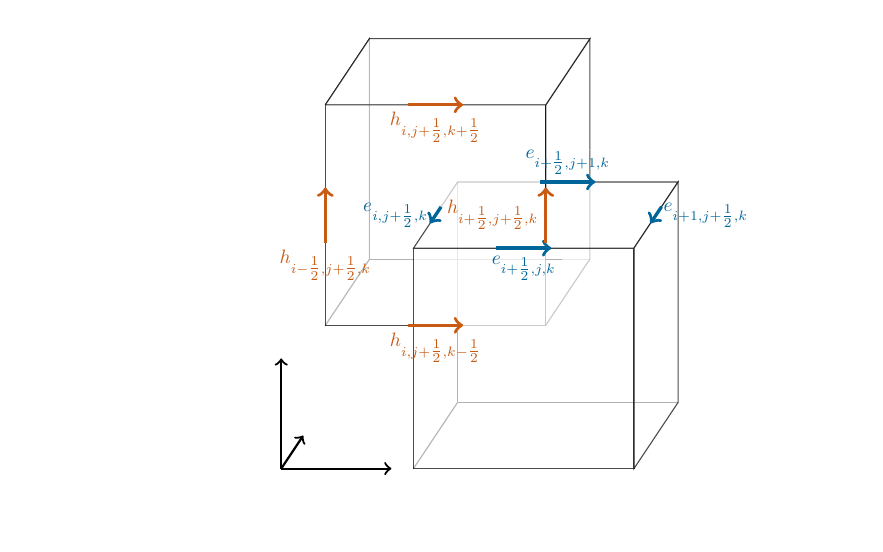
\begin{tikzpicture}[scale=0.7, every node/.style={transform shape}]
        \def\dxx{2};
        \def\dxy{0};
        \def\dyx{0.4};
        \def\dyy{0.6};
        \def\dzx{0};
        \def\dzy{2};
  \def\bgx{-7};
  \def\bgxx{8};
  \def\bgy{-5}
  \def\bgyy{4}
  \fill[opacity=0.] (\bgx,\bgy)rectangle(\bgxx,\bgyy);
        %red invisible
        \draw (-\dxx+3*\dyx-\dzx,-\dxy+3*\dyy-\dzy)
        --++(2*\dzx,2*\dzy);
        \draw (-\dxx+3*\dyx-\dzx,-\dxy+3*\dyy-\dzy)
        --++(2*\dxx,2*\dxy);
        \draw (-\dxx+3*\dyx-\dzx,-\dxy+3*\dyy-\dzy)
        --++(-2*\dyx,-2*\dyy);
        %blue invisible
        \draw (2*\dyx,2*\dyy)
        --++(-2*\dzx,-2*\dzy);
        \draw (2*\dyx-2*\dzx,2*\dyy-2*\dzy)
        --++(-2*\dyx,-2*\dyy);
        \draw (2*\dyx-2*\dzx,2*\dyy-2*\dzy)
        --++(2*\dxx,2*\dxy);
        \draw[fill=white,opacity=0.7] (\dyx-\dzy,\dyy-\dzy)
        --++(2*\dyx,2*\dyy)%--++(-\dzx,-\dzy)
        --++(2*\dzx,2*\dzy)
        --++(-2*\dyx,-2*\dyy);
        \draw[fill=white,opacity=0.7] (2*\dxx+\dyx-\dzy,2*\dxy+\dyy-\dzy)
        --++(2*\dyx,2*\dyy)%--++(-\dzx,-\dzy)
        --++(\dzx,\dzy);
        \draw[fill=white,opacity=0.7] (-\dxx+\dyx,-\dxy+\dyy)
        --++(-\dzx,-\dzy)%--++(-\dzx,-\dzy)
        --++(2*\dxx,2*\dxy)
        --++(\dzx,\dzy);
        \draw[fill=white,opacity=0.7] (2*\dxx+\dyx,2*\dxy+\dyy)
        --++(\dyx,\dyy)
        --++(-\dxx,-\dxy)--++(-\dxx,-\dxy)
        --++(-\dyx,-\dyy);
        \draw[fill=white,opacity=0.7] (-\dxx+\dyx,-\dxy+\dyy)
        --++(\dzx,\dzy)%--++(\dzx,\dzy)
        --++(\dxx,\dxy)--++(\dxx,\dxy)
        --++(-\dzx,-\dzy);%--++(-\dzx,-\dzy)
        \draw[fill=white,opacity=0.7] (\dxx+\dyx,\dxy+\dyy)
        --++(\dzx,\dzy)%--++(-\dzx,-\dzy)
        --++(2*\dyx,2*\dyy)
        --++(-\dzx,-\dzy);
        \draw[fill=white,opacity=0.7] (2*\dxx+\dyx,2*\dxy+\dyy)
        --++(-\dyx,-\dyy)
        --++(-\dxx,-\dxy)--++(-\dxx,-\dxy)
        --++(\dyx,\dyy);
        %red top 
        \draw[fill=white,opacity=0.7] (-\dxx+\dzx+\dyx,-\dxy+\dzy+\dyy)
        --++(2*\dxx,2*\dxy)
        --++(2*\dyx,2*\dyy)
        --++(-2*\dxx,-2*\dxy)
        --++(-2*\dyx,-2*\dyy);

        %blue front, right
        \draw[fill=white,opacity=0.7] (0,0)
        --++(2*\dxx,2*\dxy)
        --++(-2*\dzx,-2*\dzy)
        --++(-2*\dxx,-2*\dxy)
        --++(2*\dzx,2*\dzy);
        \draw[fill=white,opacity=0.7] (2*\dxx,2*\dxy)
        --++(2*\dyx,2*\dyy)
        --++(-2*\dzx,-2*\dzy)
        --++(-2*\dyx,-2*\dyy)
        --++(2*\dzx,2*\dzy);



        \draw[emph1,->,very thick] (1.25*\dyx,1.25*\dyy)--node[left]{$e_{i,j+\tfrac{1}{2},k}$}++(-0.5*\dyx,-0.5*\dyy);
        \draw[emph1,->,very thick] (1.25*\dyx+2*\dxx,1.25*\dyy+2*\dxy)--node[right]{$e_{i+1,j+\tfrac{1}{2},k}$}++(-0.5*\dyx,-0.5*\dyy);
%        \draw[emph1,->,very thick] (1.25*\dyx-2*\dzx,1.25*\dyy-2*\dzy)--++(-0.5*\dyx,-0.5*\dyy);
%        \draw[emph1,->,very thick] (1.25*\dyx-2*\dzx+2*\dxx,1.25*\dyy-2*\dzy+2*\dxy)--++(-0.5*\dyx,-0.5*\dyy);
%
        \draw[emph1,->,very thick] (0.75*\dxx,0.75*\dxy)--node[below]{$e_{i+\tfrac{1}{2},j,k}$}++(0.5*\dxx,0.5*\dxy);
        \draw[emph1,->,very thick] (0.75*\dxx+2*\dyx,0.75*\dxy+2*\dyy)--node[above]{$e_{i+\tfrac{1}{2},j+1,k}$}++(0.5*\dxx,0.5*\dxy);
%        \draw[emph1,->,very thick] (0.75*\dxx+2*\dyx-2*\dzx,0.75*\dxy+2*\dyy-2*\dzy)--++(0.5*\dxx,0.5*\dxy);
%        \draw[emph1,->,very thick] (0.75*\dxx-2*\dzx,0.75*\dxy-2*\dzy)--++(0.5*\dxx,0.5*\dxy);
%
%        \draw[emph1,->,very thick] (-1.25*\dzx,-1.25*\dzy)--++(0.5*\dzx,0.5*\dzy);
%        \draw[emph1,->,very thick] (-1.25*\dzx+2*\dxx,2*\dxy-1.25*\dzy)--++(0.5*\dzx,0.5*\dzy);
%        \draw[emph1,->,very thick] (-1.25*\dzx+2*\dxx+2*\dyx,2*\dxy-1.25*\dzy+2*\dyy)--++(0.5*\dzx,0.5*\dzy);
%        \draw[emph1,->,very thick] (-1.25*\dzx+2*\dyx,-1.25*\dzy+2*\dyy)--++(0.5*\dzx,0.5*\dzy);
        \begin{scope}[shift={(-\dxx+\dyx+\dzx,-\dxy+\dyy+\dzy)}]
%          \draw[emph2,->,very thick] (1.25*\dyx,1.25*\dyy)--++(-0.5*\dyx,-0.5*\dyy);
%          \draw[emph2,->,very thick] (1.25*\dyx+2*\dxx,1.25*\dyy+2*\dxy)--++(-0.5*\dyx,-0.5*\dyy);
%          \draw[emph2,->,very thick] (1.25*\dyx-2*\dzx,1.25*\dyy-2*\dzy)--++(-0.5*\dyx,-0.5*\dyy);
%          \draw[emph2,->,very thick] (1.25*\dyx-2*\dzx+2*\dxx,1.25*\dyy-2*\dzy+2*\dxy)--++(-0.5*\dyx,-0.5*\dyy);
%
          \draw[emph2,->,very thick] (0.75*\dxx,0.75*\dxy)--node[below]{$h_{i,j+\tfrac{1}{2},k+\tfrac{1}{2}}$}++(0.5*\dxx,0.5*\dxy);
%          \draw[emph2,->,very thick] (0.75*\dxx+2*\dyx,0.75*\dxy+2*\dyy)--++(0.5*\dxx,0.5*\dxy);
%          \draw[emph2,->,very thick] (0.75*\dxx+2*\dyx-2*\dzx,0.75*\dxy+2*\dyy-2*\dzy)--++(0.5*\dxx,0.5*\dxy);
          \draw[emph2,->,very thick] (0.75*\dxx-2*\dzx,0.75*\dxy-2*\dzy)--node[below]{$h_{i,j+\tfrac{1}{2},k-\tfrac{1}{2}}$}++(0.5*\dxx,0.5*\dxy);
%
          \draw[emph2,->,very thick] (-1.25*\dzx,-1.25*\dzy)node[below]{$h_{i-\tfrac{1}{2},j+\tfrac{1}{2},k}$}--++(0.5*\dzx,0.5*\dzy);
          \draw[emph2,->,very thick] (-1.25*\dzx+2*\dxx,2*\dxy-1.25*\dzy)--node[left]{$h_{i+\tfrac{1}{2},j+\tfrac{1}{2},k}$}++(0.5*\dzx,0.5*\dzy);
%          \draw[emph2,->,very thick] (-1.25*\dzx+2*\dxx+2*\dyx,2*\dxy-1.25*\dzy+2*\dyy)--++(0.5*\dzx,0.5*\dzy);
%          \draw[emph2,->,very thick] (-1.25*\dzx+2*\dyx,-1.25*\dzy+2*\dyy)--++(0.5*\dzx,0.5*\dzy);
        \end{scope}

        %\draw[gray, dashed] (.5,-5)--(0.5,1)--(2.5,4)--(2.5,-2)--(.5,-5);
        \draw[thick,->](-1.2*\dxx,-2*\dzy)--++(\dxx,\dxy);
        \draw[thick,->](-1.2*\dxx,-2*\dzy)--++(\dyx,\dyy);
        \draw[thick,->](-1.2*\dxx,-2*\dzy)--++(\dzx,\dzy);
      \end{tikzpicture}

\tikzsetnextfilename{fdtd_2d}
  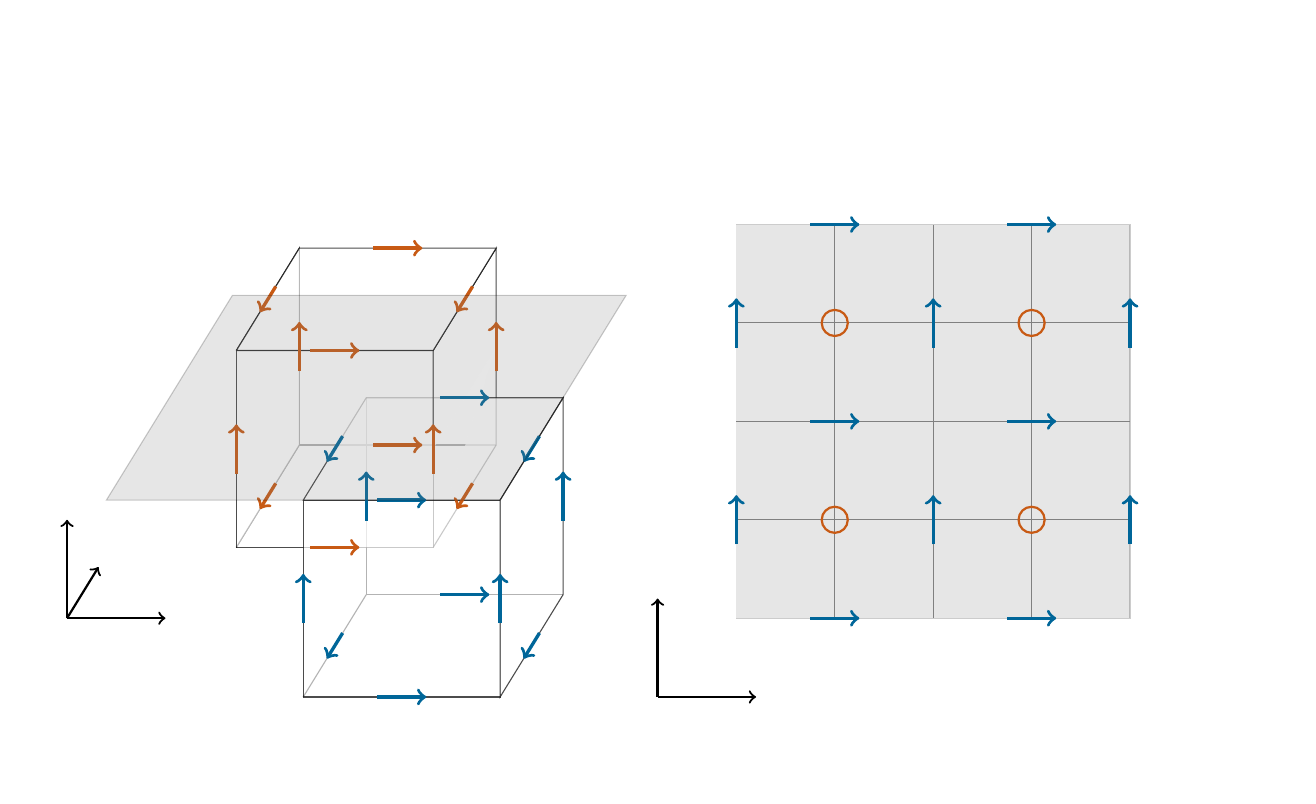
\begin{tikzpicture}[scale=0.5]
    \def\dxx{2.5};
    \def\dxy{0};
    \def\dyx{0.8};
    \def\dyy{1.3};
    \def\dzx{0};
    \def\dzy{2.5};
  \def\bgx{-7};
  \def\bgxx{25};
  \def\bgy{-7};
  \def\bgyy{12};
  \fill[opacity=0.] (\bgx,\bgy)rectangle(\bgxx,\bgyy);
    %red invisible
    \draw (-\dxx+3*\dyx-\dzx,-\dxy+3*\dyy-\dzy)
    --++(2*\dzx,2*\dzy);
    \draw (-\dxx+3*\dyx-\dzx,-\dxy+3*\dyy-\dzy)
    --++(2*\dxx,2*\dxy);
    \draw (-\dxx+3*\dyx-\dzx,-\dxy+3*\dyy-\dzy)
    --++(-2*\dyx,-2*\dyy);
    %blue invisible
    \draw (2*\dyx,2*\dyy)
    --++(-2*\dzx,-2*\dzy);
    \draw (2*\dyx-2*\dzx,2*\dyy-2*\dzy)
    --++(-2*\dyx,-2*\dyy);
    \draw (2*\dyx-2*\dzx,2*\dyy-2*\dzy)
    --++(2*\dxx,2*\dxy);
    \draw[fill=white,opacity=0.7] (\dyx-\dzy,\dyy-\dzy)
    --++(2*\dyx,2*\dyy)%--++(-\dzx,-\dzy)
    --++(2*\dzx,2*\dzy)
    --++(-2*\dyx,-2*\dyy);
    \draw[fill=white,opacity=0.7] (2*\dxx+\dyx-\dzy,2*\dxy+\dyy-\dzy)
    --++(2*\dyx,2*\dyy)%--++(-\dzx,-\dzy)
    --++(\dzx,\dzy);
    \draw[fill=white,opacity=0.7] (-\dxx+\dyx,-\dxy+\dyy)
    --++(-\dzx,-\dzy)%--++(-\dzx,-\dzy)
    --++(2*\dxx,2*\dxy)
    --++(\dzx,\dzy);
    \draw[fill=white,opacity=0.7] (2*\dxx+\dyx,2*\dxy+\dyy)
    --++(\dyx,\dyy)
    --++(-\dxx,-\dxy)--++(-\dxx,-\dxy)
    --++(-\dyx,-\dyy);
    \draw[fill=white,opacity=0.7] (-\dxx+\dyx,-\dxy+\dyy)
    --++(\dzx,\dzy)%--++(\dzx,\dzy)
    --++(\dxx,\dxy)--++(\dxx,\dxy)
    --++(-\dzx,-\dzy);%--++(-\dzx,-\dzy)
    \draw[fill=white,opacity=0.7] (\dxx+\dyx,\dxy+\dyy)
    --++(\dzx,\dzy)%--++(-\dzx,-\dzy)
    --++(2*\dyx,2*\dyy)
    --++(-\dzx,-\dzy);
    \draw[fill=white,opacity=0.7] (2*\dxx+\dyx,2*\dxy+\dyy)
    --++(-\dyx,-\dyy)
    --++(-\dxx,-\dxy)--++(-\dxx,-\dxy)
    --++(\dyx,\dyy);
    %red top 
    \draw[fill=white,opacity=0.7] (-\dxx+\dzx+\dyx,-\dxy+\dzy+\dyy)
    --++(2*\dxx,2*\dxy)
    --++(2*\dyx,2*\dyy)
    --++(-2*\dxx,-2*\dxy)
    --++(-2*\dyx,-2*\dyy);

    %blue front, right
    \draw[fill=white,opacity=0.7] (0,0)
    --++(2*\dxx,2*\dxy)
    --++(-2*\dzx,-2*\dzy)
    --++(-2*\dxx,-2*\dxy)
    --++(2*\dzx,2*\dzy);
    \draw[fill=white,opacity=0.7] (2*\dxx,2*\dxy)
    --++(2*\dyx,2*\dyy)
    --++(-2*\dzx,-2*\dzy)
    --++(-2*\dyx,-2*\dyy)
    --++(2*\dzx,2*\dzy);
  


    \draw[emph1,->,very thick] (1.25*\dyx,1.25*\dyy)--++(-0.5*\dyx,-0.5*\dyy);
    \draw[emph1,->,very thick] (1.25*\dyx+2*\dxx,1.25*\dyy+2*\dxy)--++(-0.5*\dyx,-0.5*\dyy);
    \draw[emph1,->,very thick] (1.25*\dyx-2*\dzx,1.25*\dyy-2*\dzy)--++(-0.5*\dyx,-0.5*\dyy);
    \draw[emph1,->,very thick] (1.25*\dyx-2*\dzx+2*\dxx,1.25*\dyy-2*\dzy+2*\dxy)--++(-0.5*\dyx,-0.5*\dyy);

    \draw[emph1,->,very thick] (0.75*\dxx,0.75*\dxy)--++(0.5*\dxx,0.5*\dxy);
    \draw[emph1,->,very thick] (0.75*\dxx+2*\dyx,0.75*\dxy+2*\dyy)--++(0.5*\dxx,0.5*\dxy);
    \draw[emph1,->,very thick] (0.75*\dxx+2*\dyx-2*\dzx,0.75*\dxy+2*\dyy-2*\dzy)--++(0.5*\dxx,0.5*\dxy);
    \draw[emph1,->,very thick] (0.75*\dxx-2*\dzx,0.75*\dxy-2*\dzy)--++(0.5*\dxx,0.5*\dxy);

    \draw[emph1,->,very thick] (-1.25*\dzx,-1.25*\dzy)--++(0.5*\dzx,0.5*\dzy);
    \draw[emph1,->,very thick] (-1.25*\dzx+2*\dxx,2*\dxy-1.25*\dzy)--++(0.5*\dzx,0.5*\dzy);
    \draw[emph1,->,very thick] (-1.25*\dzx+2*\dxx+2*\dyx,2*\dxy-1.25*\dzy+2*\dyy)--++(0.5*\dzx,0.5*\dzy);
    \draw[emph1,->,very thick] (-1.25*\dzx+2*\dyx,-1.25*\dzy+2*\dyy)--++(0.5*\dzx,0.5*\dzy);
    \begin{scope}[shift={(-\dxx+\dyx+\dzx,-\dxy+\dyy+\dzy)}]
    \draw[emph2,->,very thick] (1.25*\dyx,1.25*\dyy)--++(-0.5*\dyx,-0.5*\dyy);
    \draw[emph2,->,very thick] (1.25*\dyx+2*\dxx,1.25*\dyy+2*\dxy)--++(-0.5*\dyx,-0.5*\dyy);
    \draw[emph2,->,very thick] (1.25*\dyx-2*\dzx,1.25*\dyy-2*\dzy)--++(-0.5*\dyx,-0.5*\dyy);
    \draw[emph2,->,very thick] (1.25*\dyx-2*\dzx+2*\dxx,1.25*\dyy-2*\dzy+2*\dxy)--++(-0.5*\dyx,-0.5*\dyy);

    \draw[emph2,->,very thick] (0.75*\dxx,0.75*\dxy)--++(0.5*\dxx,0.5*\dxy);
    \draw[emph2,->,very thick] (0.75*\dxx+2*\dyx,0.75*\dxy+2*\dyy)--++(0.5*\dxx,0.5*\dxy);
    \draw[emph2,->,very thick] (0.75*\dxx+2*\dyx-2*\dzx,0.75*\dxy+2*\dyy-2*\dzy)--++(0.5*\dxx,0.5*\dxy);
    \draw[emph2,->,very thick] (0.75*\dxx-2*\dzx,0.75*\dxy-2*\dzy)--++(0.5*\dxx,0.5*\dxy);

    \draw[emph2,->,very thick] (-1.25*\dzx,-1.25*\dzy)--++(0.5*\dzx,0.5*\dzy);
    \draw[emph2,->,very thick] (-1.25*\dzx+2*\dxx,2*\dxy-1.25*\dzy)--++(0.5*\dzx,0.5*\dzy);
    \draw[emph2,->,very thick] (-1.25*\dzx+2*\dxx+2*\dyx,2*\dxy-1.25*\dzy+2*\dyy)--++(0.5*\dzx,0.5*\dzy);
    \draw[emph2,->,very thick] (-1.25*\dzx+2*\dyx,-1.25*\dzy+2*\dyy)--++(0.5*\dzx,0.5*\dzy);
    \end{scope}
    
    \draw[fill=gray,opacity=0.2] (2*\dxx,2*\dxy)
    --++(4*\dyx,4*\dyy)
    --++(-4*\dxx,-4*\dxy)
    --++(-4*\dyx,-4*\dyy)
    --++(4*\dxx,4*\dxy);

    %\draw[gray, dashed] (.5,-5)--(0.5,1)--(2.5,4)--(2.5,-2)--(.5,-5);
    \draw[thick,->](-6,-3)--++(\dxx,\dxy);
    \draw[thick,->](-6,-3)--++(\dyx,\dyy);
    \draw[thick,->](-6,-3)--++(\dzx,\dzy);
    \begin{scope}[shift={(11,-3)}]
    \def\dx{2.5};
    \def\dy{2.5};
    \draw[fill=gray,opacity=0.2] (0,0)--++(4*\dx,0)--++(0,4*\dy)--++(-4*\dx,0);
    \draw[gray] (\dx,0)--++(0,4*\dy);
    \draw[gray] (2*\dx,0)--++(0,4*\dy);
    \draw[gray] (3*\dx,0)--++(0,4*\dy);
    \draw[gray] (0,\dy)--++(4*\dx,0);
    \draw[gray] (0,2*\dy)--++(4*\dx,0);
    \draw[gray] (0,3*\dy)--++(4*\dx,0);

    \draw[emph1,->,very thick] (\dx-0.25*\dx,0)--++(0.5*\dx,0);
    \draw[emph1,->,very thick] (3*\dx-0.25*\dx,0)--++(0.5*\dx,0);


    \draw[emph1,->,very thick] (\dx-0.25*\dx,2*\dy)--++(0.5*\dx,0);
    \draw[emph1,->,very thick] (3*\dx-0.25*\dx,2*\dy)--++(0.5*\dx,0);


    \draw[emph1,->,very thick] (\dx-0.25*\dx,4*\dy)--++(0.5*\dx,0);
    \draw[emph1,->,very thick] (3*\dx-0.25*\dx,4*\dy)--++(0.5*\dx,0);

    \draw[emph1,->,very thick] (0,\dy-0.25*\dy)--++(0,0.5*\dy);
    \draw[emph1,->,very thick] (0,3*\dy-0.25*\dy,0)--++(0,0.5*\dy);

    \draw[emph1,->,very thick] (2*\dx,\dy-0.25*\dy)--++(0,0.5*\dy);
    \draw[emph1,->,very thick] (2*\dx,3*\dy-0.25*\dy,0)--++(0,0.5*\dy);

    \draw[emph1,->,very thick] (4*\dx,\dy-0.25*\dy)--++(0,0.5*\dy);
    \draw[emph1,->,very thick] (4*\dx,3*\dy-0.25*\dy,0)--++(0,0.5*\dy);

    \node[circle,thick,draw=emph2] at (\dx,\dy){};
    \node[circle,thick,draw=emph2] at (3*\dx,\dy){};
    \node[circle,thick,draw=emph2] at (\dx,3*\dy){};
    \node[circle,thick,draw=emph2] at (3*\dx,3*\dy){};
    %axis
    \draw[thick,->](-2,-2)--++(\dx,0);
    \draw[thick,->](-2,-2)--++(0,\dy);
    \end{scope}
  \end{tikzpicture}
      

\tikzsetnextfilename{primal_dual_quad}
  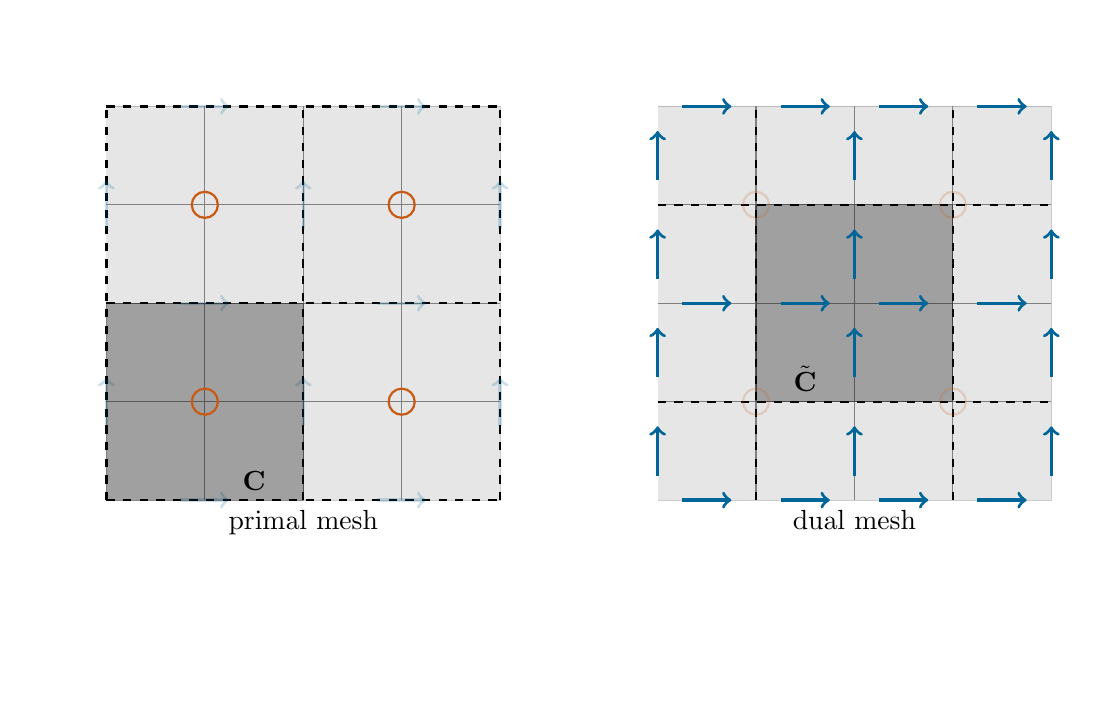
\begin{tikzpicture}[scale=0.5]
    \def\dx{2.5};
    \def\dy{2.5};
  \def\bgx{-2};
  \def\bgxx{25};
  \def\bgy{-5};
  \def\bgyy{12};
  \fill[opacity=0.] (\bgx,\bgy)rectangle(\bgxx,\bgyy);
    \draw[fill=gray,opacity=0.2] (0,0)--++(4*\dx,0)--++(0,4*\dy)--++(-4*\dx,0);
    \draw[gray] (\dx,0)--++(0,4*\dy);
    \draw[gray] (2*\dx,0)--++(0,4*\dy);
    \draw[gray] (3*\dx,0)--++(0,4*\dy);
    \draw[gray] (0,\dy)--++(4*\dx,0);
    \draw[gray] (0,2*\dy)--++(4*\dx,0);
    \draw[gray] (0,3*\dy)--++(4*\dx,0);

    \draw[black,thick,dashed] (0,0)--++(4*\dx,0);
    \draw[black,thick,dashed] (0,0)--++(0,4*\dy);
    \draw[black,thick,dashed] (2*\dx,0)--++(0,4*\dy);
    \draw[black,thick,dashed] (4*\dx,0)--++(0,4*\dy);
    \draw[black,thick,dashed] (0,2*\dy)--++(4*\dx,0);
    \draw[black,thick,dashed] (0,4*\dy)--++(4*\dx,0);



    \draw[emph1,->,very thick,opacity=0.2] (\dx-0.25*\dx,0)--++(0.5*\dx,0);
    \draw[emph1,->,very thick,opacity=0.2] (3*\dx-0.25*\dx,0)--++(0.5*\dx,0);
    \draw[emph1,->,very thick,opacity=0.2] (\dx-0.25*\dx,2*\dy)--++(0.5*\dx,0);
    \draw[emph1,->,very thick,opacity=0.2] (3*\dx-0.25*\dx,2*\dy)--++(0.5*\dx,0);
    \draw[emph1,->,very thick,opacity=0.2] (\dx-0.25*\dx,4*\dy)--++(0.5*\dx,0);
    \draw[emph1,->,very thick,opacity=0.2] (3*\dx-0.25*\dx,4*\dy)--++(0.5*\dx,0);
    \draw[emph1,->,very thick,opacity=0.2] (0,\dy-0.25*\dy)--++(0,0.5*\dy);
    \draw[emph1,->,very thick,opacity=0.2] (0,3*\dy-0.25*\dy,0)--++(0,0.5*\dy);
    \draw[emph1,->,very thick,opacity=0.2] (2*\dx,\dy-0.25*\dy)--++(0,0.5*\dy);
    \draw[emph1,->,very thick,opacity=0.2] (2*\dx,3*\dy-0.25*\dy,0)--++(0,0.5*\dy);
    \draw[emph1,->,very thick,opacity=0.2] (4*\dx,\dy-0.25*\dy)--++(0,0.5*\dy);
    \draw[emph1,->,very thick,opacity=0.2] (4*\dx,3*\dy-0.25*\dy,0)--++(0,0.5*\dy);
    \draw[fill=black,opacity=0.3](0,0)--++(2*\dx,0)--++(0,2*\dy)--++(-2*\dx,0)--++(0,-2*\dy);
    \node[above] at (1.5*\dx,0){$\mathbf C$};
    \node[circle,thick,draw=emph2] at (\dx,\dy){};
    \node[circle,thick,draw=emph2] at (3*\dx,\dy){};
    \node[circle,thick,draw=emph2] at (\dx,3*\dy){};
    \node[circle,thick,draw=emph2] at (3*\dx,3*\dy){};
    \node[below] at (2*\dx,0){primal mesh};
    \begin{scope}[shift={(14,0)}]
    \def\dx{2.5};
    \def\dy{2.5};
    \draw[fill=gray,opacity=0.2] (0,0)--++(4*\dx,0)--++(0,4*\dy)--++(-4*\dx,0);
    \draw[gray] (\dx,0)--++(0,4*\dy);
    \draw[gray] (2*\dx,0)--++(0,4*\dy);
    \draw[gray] (3*\dx,0)--++(0,4*\dy);
    \draw[gray] (0,\dy)--++(4*\dx,0);
    \draw[gray] (0,2*\dy)--++(4*\dx,0);
    \draw[gray] (0,3*\dy)--++(4*\dx,0);

    \draw[black,thick,dashed] (1*\dx,0)--++(0,4*\dy);
    \draw[black,thick,dashed] (3*\dx,0)--++(0,4*\dy);
    \draw[black,thick,dashed] (0,1*\dy)--++(4*\dx,0);
    \draw[black,thick,dashed] (0,3*\dy)--++(4*\dx,0);
    \draw[fill=black,opacity=0.3](\dx,\dy)--++(2*\dx,0)--++(0,2*\dy)--++(-2*\dx,0)--++(0,-2*\dy);
    \node[above] at (1.5*\dx,1*\dy){$\tilde {\mathbf C}$};

    \draw[emph1,->,very thick] (0.5*\dx-0.25*\dx,0)--++(0.5*\dx,0);
    \draw[emph1,->,very thick] (1.5*\dx-0.25*\dx,0)--++(0.5*\dx,0);
    \draw[emph1,->,very thick] (2.5*\dx-0.25*\dx,0)--++(0.5*\dx,0);
    \draw[emph1,->,very thick] (3.5*\dx-0.25*\dx,0)--++(0.5*\dx,0);
    \draw[emph3,->,very thick,opacity=0] (\dx-0.25*\dx,0)--++(0.5*\dx,0);
    \draw[emph3,->,very thick,opacity=0] (3.5*\dx-0.25*\dx,4*\dy)--++(0.5*\dx,0);

    \draw[emph1,->,very thick] (0.5*\dx-0.25*\dx,2*\dy)--++(0.5*\dx,0);
    \draw[emph1,->,very thick] (1.5*\dx-0.25*\dx,2*\dy)--++(0.5*\dx,0);
    \draw[emph1,->,very thick] (2.5*\dx-0.25*\dx,2*\dy)--++(0.5*\dx,0);
    \draw[emph1,->,very thick] (3.5*\dx-0.25*\dx,2*\dy)--++(0.5*\dx,0);

    \draw[emph1,->,very thick] (0.5*\dx-0.25*\dx,4*\dy)--++(0.5*\dx,0);
    \draw[emph1,->,very thick] (1.5*\dx-0.25*\dx,4*\dy)--++(0.5*\dx,0);
    \draw[emph1,->,very thick] (2.5*\dx-0.25*\dx,4*\dy)--++(0.5*\dx,0);
    \draw[emph1,->,very thick] (3.5*\dx-0.25*\dx,4*\dy)--++(0.5*\dx,0);

    \draw[emph1,->,very thick] (0,0.5*\dy-0.25*\dy)--++(0,0.5*\dy);
    \draw[emph1,->,very thick] (0,1.5*\dy-0.25*\dy)--++(0,0.5*\dy);
    \draw[emph1,->,very thick] (0,2.5*\dy-0.25*\dy)--++(0,0.5*\dy);
    \draw[emph1,->,very thick] (0,3.5*\dy-0.25*\dy,0)--++(0,0.5*\dy);

    \draw[emph1,->,very thick] (2*\dx,0.5*\dy-0.25*\dy)--++(0,0.5*\dy);
    \draw[emph1,->,very thick] (2*\dx,1.5*\dy-0.25*\dy)--++(0,0.5*\dy);
    \draw[emph1,->,very thick] (2*\dx,2.5*\dy-0.25*\dy)--++(0,0.5*\dy);
    \draw[emph1,->,very thick] (2*\dx,3.5*\dy-0.25*\dy,0)--++(0,0.5*\dy);

    \draw[emph1,->,very thick] (4*\dx,0.5*\dy-0.25*\dy)--++(0,0.5*\dy);
    \draw[emph1,->,very thick] (4*\dx,1.5*\dy-0.25*\dy)--++(0,0.5*\dy);
    \draw[emph1,->,very thick] (4*\dx,2.5*\dy-0.25*\dy)--++(0,0.5*\dy);
    \draw[emph1,->,very thick] (4*\dx,3.5*\dy-0.25*\dy,0)--++(0,0.5*\dy);

    \node[circle,thick,draw=emph2,opacity=0.2] at (\dx,\dy){};
    \node[circle,thick,draw=emph2,opacity=0.2] at (3*\dx,\dy){};
    \node[circle,thick,draw=emph2,opacity=0.2] at (\dx,3*\dy){};
    \node[circle,thick,draw=emph2,opacity=0.2] at (3*\dx,3*\dy){};
    %axis
    %\draw[thick,->](-2,-2)--++(\dx,0);
    %\draw[thick,->](-2,-2)--++(0,\dy);
    \node[below] at (2*\dx,0){dual mesh};
    \end{scope}
  \end{tikzpicture}%

\tikzsetnextfilename{barycentric}

\newcommand\trignew[6]{\draw[thick](#1,#2)--(#3,#4)--(#5,#6)--cycle;
\draw(0.5*#1+0.5*#3,0.5*#2+0.5*#4)--(1/3*#1+1/3*#3+1/3*#5,1/3*#2+1/3*#4+1/3*#6);
\draw(0.5*#1+0.5*#5,0.5*#2+0.5*#6)--(1/3*#1+1/3*#3+1/3*#5,1/3*#2+1/3*#4+1/3*#6);
\draw(0.5*#3+0.5*#5,0.5*#4+0.5*#6)--(1/3*#1+1/3*#3+1/3*#5,1/3*#2+1/3*#4+1/3*#6);}
\newcommand\trigfilled[6]{\draw[thick,fill=emph2,opacity=0.2](#1,#2)--(#3,#4)--(#5,#6)--node[above right,opacity=1]{$T_i$}cycle;}

  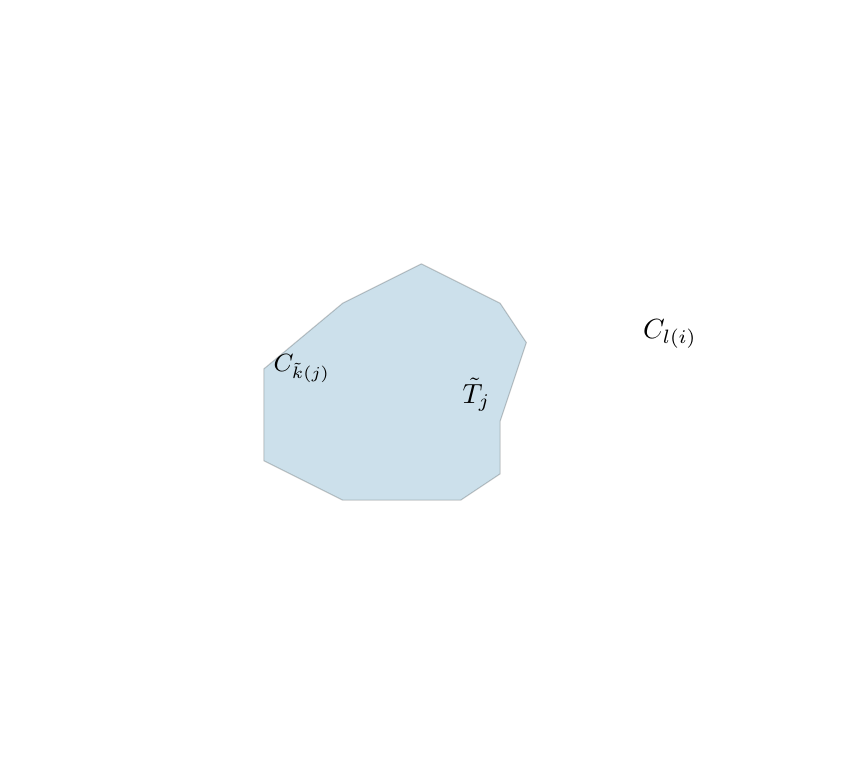
\begin{tikzpicture}
    \def\ax{0};
    \def\ay{-1};
    \def\bx{3};
    \def\by{0};
    \def\cx{1};
    \def\cy{1};
    \def\dx{3};
    \def\dy{2};
    \def\ex{1};
    \def\ey{4};
    \def\fx{-1};
    \def\fy{1};
    \def\gx{-3};
    \def\gy{4};
    \def\hx{-5};
    \def\hy{0};
  \def\bgx{-6};
  \def\bgxx{4};
  \def\bgy{-3};
  \def\bgyy{6};
  \fill[opacity=0.] (\bgx,\bgy)rectangle(\bgxx,\bgyy);
    \trignew{\ax}{\ay}{\bx}{\by}{\cx}{\cy};
    \trignew{\bx}{\by}{\cx}{\cy}{\dx}{\dy};
    \trignew{\cx}{\cy}{\dx}{\dy}{\ex}{\ey};
    \trignew{\cx}{\cy}{\fx}{\fy}{\ex}{\ey};
    \trignew{\cx}{\cy}{\fx}{\fy}{\ax}{\ay};
    \trignew{\gx}{\gy}{\fx}{\fy}{\ex}{\ey};
    \trignew{\gx}{\gy}{\fx}{\fy}{\hx}{\hy};
    \trignew{\ax}{\ay}{\fx}{\fy}{\hx}{\hy};
    %dual cell
    \draw[fill=emph1,opacity=0.2](0.5*\hx+0.5*\fx,0.5*\hy+0.5*\fy)
    --(1/3*\gx+1/3*\fx+1/3*\hx,1/3*\gy+1/3*\fy+1/3*\hy)node[right,opacity=1]{\small${C}_{\tilde k(j)}$}
    --(0.5*\gx+0.5*\fx,0.5*\gy+0.5*\fy)
    --(1/3*\gx+1/3*\fx+1/3*\ex,1/3*\gy+1/3*\fy+1/3*\ey)
    --(0.5*\ex+0.5*\fx,0.5*\ey+0.5*\fy)
    --(1/3*\ex+1/3*\fx+1/3*\cx,1/3*\cy+1/3*\fy+1/3*\ey)
    --(0.5*\cx+0.5*\fx,0.5*\cy+0.5*\fy)node[above left,opacity=1]{$\tilde{T}_j$}
    --(1/3*\ax+1/3*\fx+1/3*\cx,1/3*\cy+1/3*\fy+1/3*\ay)
    --(0.5*\ax+0.5*\fx,0.5*\ay+0.5*\fy)
    --(1/3*\ax+1/3*\fx+1/3*\hx,1/3*\hy+1/3*\fy+1/3*\ay)--cycle;
    %mapped quad dual
    %primal cell
    \trigfilled{\cx}{\cy}{\dx}{\dy}{\ex}{\ey};
    %mapped quad primal
    %comment \varphi
    %ref dual
    \node[] at (1/9*\cx+1/9*\dx+1/9*\ex+2/3*\dx-0.4,1/9*\cy+1/9*\dy+1/9*\ey+2/3*\dy){$C_{l(i)}$};
  \end{tikzpicture}

\tikzsetnextfilename{mapping_primal_h1}


  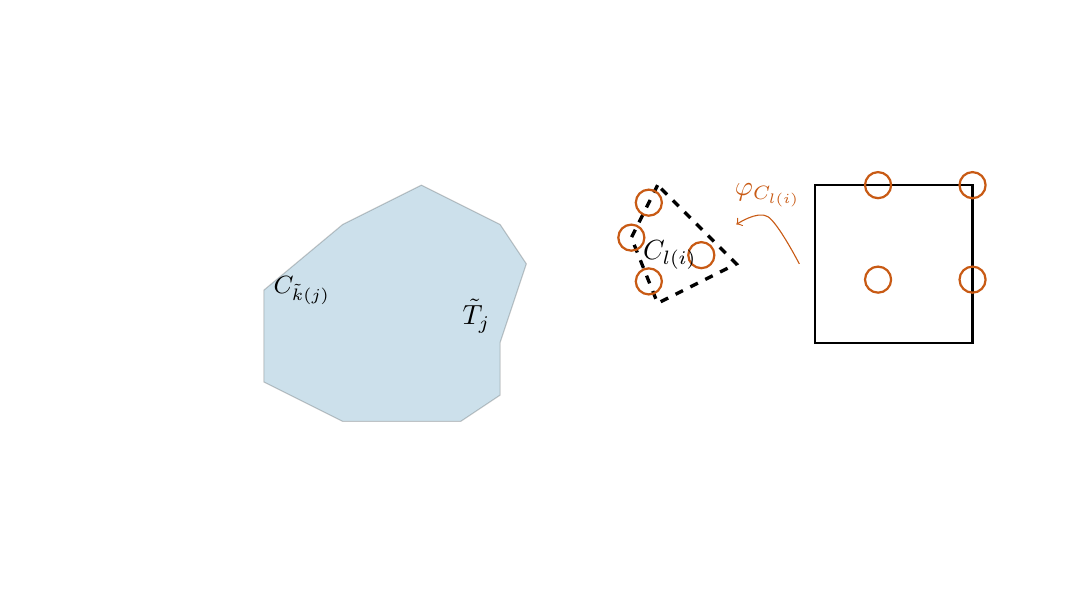
\begin{tikzpicture}
    \def\ax{0};
    \def\ay{-1};
    \def\bx{3};
    \def\by{0};
    \def\cx{1};
    \def\cy{1};
    \def\dx{3};
    \def\dy{2};
    \def\ex{1};
    \def\ey{4};
    \def\fx{-1};
    \def\fy{1};
    \def\gx{-3};
    \def\gy{4};
    \def\hx{-5};
    \def\hy{0};
  \def\bgx{-6};
  \def\bgxx{7};
  \def\bgy{-2};
  \def\bgyy{5};
  \fill[opacity=0.] (\bgx,\bgy)rectangle(\bgxx,\bgyy);
    \trignew{\ax}{\ay}{\bx}{\by}{\cx}{\cy};
    \trignew{\bx}{\by}{\cx}{\cy}{\dx}{\dy};
    \trignew{\cx}{\cy}{\dx}{\dy}{\ex}{\ey};
    \trignew{\cx}{\cy}{\fx}{\fy}{\ex}{\ey};
    \trignew{\cx}{\cy}{\fx}{\fy}{\ax}{\ay};
    \trignew{\gx}{\gy}{\fx}{\fy}{\ex}{\ey};
    \trignew{\gx}{\gy}{\fx}{\fy}{\hx}{\hy};
    \trignew{\ax}{\ay}{\fx}{\fy}{\hx}{\hy};
    %dual cell
    \draw[fill=emph1,opacity=0.2](0.5*\hx+0.5*\fx,0.5*\hy+0.5*\fy)
    --(1/3*\gx+1/3*\fx+1/3*\hx,1/3*\gy+1/3*\fy+1/3*\hy)node[right,opacity=1]{\small${C}_{\tilde k(j)}$}
    --(0.5*\gx+0.5*\fx,0.5*\gy+0.5*\fy)
    --(1/3*\gx+1/3*\fx+1/3*\ex,1/3*\gy+1/3*\fy+1/3*\ey)
    --(0.5*\ex+0.5*\fx,0.5*\ey+0.5*\fy)
    --(1/3*\ex+1/3*\fx+1/3*\cx,1/3*\cy+1/3*\fy+1/3*\ey)
    --(0.5*\cx+0.5*\fx,0.5*\cy+0.5*\fy)node[above left,opacity=1]{$\tilde{T}_j$}
    --(1/3*\ax+1/3*\fx+1/3*\cx,1/3*\cy+1/3*\fy+1/3*\ay)
    --(0.5*\ax+0.5*\fx,0.5*\ay+0.5*\fy)
    --(1/3*\ax+1/3*\fx+1/3*\hx,1/3*\hy+1/3*\fy+1/3*\ay)--cycle;
    %mapped quad dual
    \draw[->,emph2]plot[smooth,tension=0.6] coordinates{ (3.8,2)(3.4,2.6)(3,2.5)};
    \node[emph2,above] at(3.4,2.6){$\varphi_{C_{l(i)}}$};
    \draw[very thick,dashed](0.5*\ex+0.5*\dx,0.5*\ey+0.5*\dy)
    --(1/3*\cx+1/3*\dx+1/3*\ex,1/3*\cy+1/3*\dy+1/3*\ey)
    --(0.5*\dx+0.5*\cx,0.5*\dy+0.5*\cy)
    --(\dx,\dy)--cycle;
    %primal cell
    \trigfilled{\cx}{\cy}{\dx}{\dy}{\ex}{\ey};
    %mapped quad primal
    %comment \varphi
    \draw[thick](4,1)--++(2,0)--++(0,2)--++(-2,0)--cycle;
    \node[circle,thick,draw=emph2] at (6,3){};
    \node[circle,thick,draw=emph2] at (4.8,3){};
    \node[circle,thick,draw=emph2] at (4.8,1.8){};
    \node[circle,thick,draw=emph2] at (6,1.8){};
    %mappofs primal
    \node[circle,thick,draw=emph2] at (1/3*\cx+1/3*\dx+1/3*\ex,1/3*\cy+1/3*\dy+1/3*\ey){};
    \node[circle,thick,draw=emph2] at (0.5*2/3*\ex+0.5*2/3*\dx+1/9*\cx+1/9*\dx+1/9*\ex,0.5*2/3*\ey+0.5*2/3*\dy+1/9*\cy+1/9*\dy+1/9*\ey){};
    \node[circle,thick,draw=emph2] at (0.5*2/3*\cx+0.5*2/3*\dx+1/9*\cx+1/9*\dx+1/9*\ex,0.5*2/3*\cy+0.5*2/3*\dy+1/9*\cy+1/9*\dy+1/9*\ey){};
    \node[circle,thick,draw=emph2] at (1/9*\cx+1/9*\dx+1/9*\ex+2/3*\dx,1/9*\cy+1/9*\dy+1/9*\ey+2/3*\dy){};
    %ref dual
    \node[] at (1/9*\cx+1/9*\dx+1/9*\ex+2/3*\dx-0.4,1/9*\cy+1/9*\dy+1/9*\ey+2/3*\dy){$C_{l(i)}$};
  \end{tikzpicture}

\tikzsetnextfilename{mapping_dual_hcurl}

  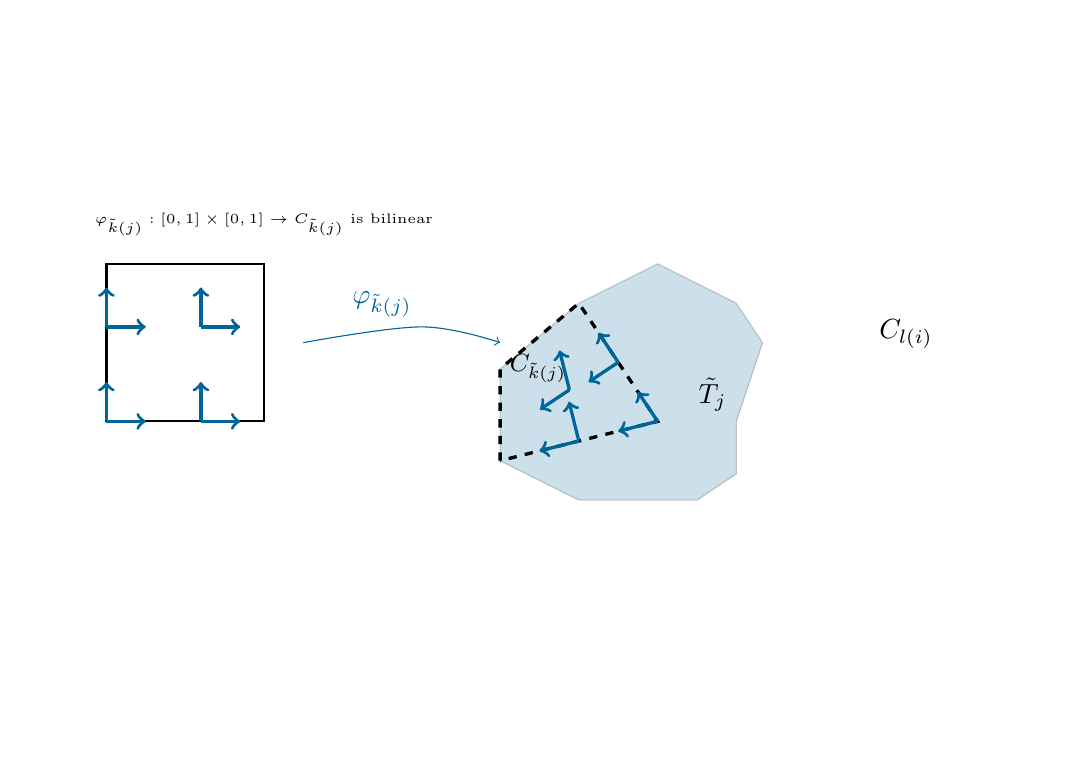
\begin{tikzpicture}
    \def\ax{0};
    \def\ay{-1};
    \def\bx{3};
    \def\by{0};
    \def\cx{1};
    \def\cy{1};
    \def\dx{3};
    \def\dy{2};
    \def\ex{1};
    \def\ey{4};
    \def\fx{-1};
    \def\fy{1};
    \def\gx{-3};
    \def\gy{4};
    \def\hx{-5};
    \def\hy{0};
  \def\bgx{-9};
  \def\bgxx{4};
  \def\bgy{-3};
  \def\bgyy{6};
  \fill[opacity=0.] (\bgx,\bgy)rectangle(\bgxx,\bgyy);
    \trignew{\ax}{\ay}{\bx}{\by}{\cx}{\cy};
    \trignew{\bx}{\by}{\cx}{\cy}{\dx}{\dy};
    \trignew{\cx}{\cy}{\dx}{\dy}{\ex}{\ey};
    \trignew{\cx}{\cy}{\fx}{\fy}{\ex}{\ey};
    \trignew{\cx}{\cy}{\fx}{\fy}{\ax}{\ay};
    \trignew{\gx}{\gy}{\fx}{\fy}{\ex}{\ey};
    \trignew{\gx}{\gy}{\fx}{\fy}{\hx}{\hy};
    \trignew{\ax}{\ay}{\fx}{\fy}{\hx}{\hy};
    %dual cell
    \draw[fill=emph1,opacity=0.2](0.5*\hx+0.5*\fx,0.5*\hy+0.5*\fy)
    --(1/3*\gx+1/3*\fx+1/3*\hx,1/3*\gy+1/3*\fy+1/3*\hy)node[right,opacity=1]{\small${C}_{\tilde k(j)}$}
    --(0.5*\gx+0.5*\fx,0.5*\gy+0.5*\fy)
    --(1/3*\gx+1/3*\fx+1/3*\ex,1/3*\gy+1/3*\fy+1/3*\ey)
    --(0.5*\ex+0.5*\fx,0.5*\ey+0.5*\fy)
    --(1/3*\ex+1/3*\fx+1/3*\cx,1/3*\cy+1/3*\fy+1/3*\ey)
    --(0.5*\cx+0.5*\fx,0.5*\cy+0.5*\fy)node[above left,opacity=1]{$\tilde{T}_j$}
    --(1/3*\ax+1/3*\fx+1/3*\cx,1/3*\cy+1/3*\fy+1/3*\ay)
    --(0.5*\ax+0.5*\fx,0.5*\ay+0.5*\fy)
    --(1/3*\ax+1/3*\fx+1/3*\hx,1/3*\hy+1/3*\fy+1/3*\ay)--cycle;
    %mapped quad dual
    \draw[very thick,dashed](0.5*\hx+0.5*\fx,0.5*\hy+0.5*\fy)
    --(1/3*\gx+1/3*\fx+1/3*\hx,1/3*\gy+1/3*\fy+1/3*\hy)
    --(0.5*\gx+0.5*\fx,0.5*\gy+0.5*\fy)
    --(\fx,\fy)--cycle;
    \draw[->,emph1]plot[smooth,tension=0.6] coordinates{ (-5.5,2)(-4,2.2)(-3,2)};
    \node[emph1,above left] at(-4,2.2){$\varphi_{\tilde k(j)}$};
    %primal cell
    \trigfilled{\cx}{\cy}{\dx}{\dy}{\ex}{\ey};
    %mapped quad primal
    %comment \varphi
    %ref dual
    \draw[thick,black](-8,1)--++(2,0)--++(0,2)--++(-2,0)--cycle;
    \draw[very thick,->,emph1](-8,1)--++(0.5,0);
    \draw[very thick,->,emph1](-8,1)--++(0,0.5);
    \draw[very thick,->,emph1](-8,2.2)--++(0.5,0);
    \draw[very thick,->,emph1](-8,2.2)--++(0,0.5);
    \draw[very thick,->,emph1](-6.8,1)--++(0,0.5);
    \draw[very thick,->,emph1](-6.8,1)--++(0.5,0);
    \draw[very thick,->,emph1](-6.8,2.2)--++(0,0.5);
    \draw[very thick,->,emph1](-6.8,2.2)--++(0.5,0);
    %dofsped dual
    \node at (-6,3.5) {\tiny$\varphi_{\tilde k(j)}:[0,1]\times[0,1]\to C_{\tilde k(j)}$ is bilinear};
    \draw[very thick,->,emph1](\fx,\fy)--++(0.125*\hx-0.125*\fx,0.125*\hy-0.125*\fy);
    \draw[very thick,->,emph1](\fx,\fy)--++(0.125*\gx-0.125*\fx,0.125*\gy-0.125*\fy);
    \draw[very thick,->,emph1](\fx+0.25*\hx-0.25*\fx,\fy+0.25*\hy-0.25*\fy)--++(0.125*\hx-0.125*\fx,0.125*\hy-0.125*\fy);
    \draw[very thick,->,emph1](\fx+0.25*\hx-0.25*\fx,\fy+0.25*\hy-0.25*\fy)--++(0.125*\hy-0.125*\fy,-0.125*\hx+0.125*\fx);
    \draw[very thick,->,emph1](\fx+0.25*\gx-0.25*\fx,\fy+0.25*\gy-0.25*\fy)--++(0.125*\gx-0.125*\fx,0.125*\gy-0.125*\fy);
    \draw[very thick,->,emph1](\fx+0.25*\gx-0.25*\fx,\fy+0.25*\gy-0.25*\fy)--++(-0.125*\gy+0.125*\fy,0.125*\gx-0.125*\fx);
    \draw[very thick,->,emph1](0.5*\fx+0.18*\gx+0.18*\fx+0.18*\hx,0.5*\fy+0.18*\gy+0.18*\fy+0.18*\hy)--++(-0.125*\gy+0.125*\fy,0.125*\gx-0.125*\fx);
    \draw[very thick,->,emph1](0.5*\fx+0.18*\gx+0.18*\fx+0.18*\hx,0.5*\fy+0.18*\gy+0.18*\fy+0.18*\hy)--++(0.125*\hy-0.125*\fy,-0.125*\hx+0.125*\fx);
    \node[] at (1/9*\cx+1/9*\dx+1/9*\ex+2/3*\dx-0.4,1/9*\cy+1/9*\dy+1/9*\ey+2/3*\dy){$C_{l(i)}$};
  \end{tikzpicture}













\newcommand\arrowdofcube[7][]{%
  \draw[emph1,-latex,very thick](#2,#3,#4)--(#5,#6,#7);
  }
\newcommand\arrowdoftet[7][]{%
  \def\x{#2/2-#2*#3/6-#2*#4/6+#2*#3*#4/12};
  \def\y{#3/2-#3*#2/6-#3*#4/6+#2*#3*#4/12};
  \def\z{#4/2-#4*#3/6-#2*#4/6+#2*#3*#4/12};
  \def\xx{#5/2-#5*#6/6-#5*#7/6+#5*#6*#7/12};
  \def\yy{#6/2-#6*#5/6-#6*#7/6+#5*#6*#7/12};
  \def\zz{#7/2-#7*#6/6-#5*#7/6+#5*#6*#7/12};
  \def\xyz{1-#2/2-#3/2-#4/2-#2*#3*#4/4+#2*#3/6+#2*#4/6+#3*#2/6+#3*#4/6+#4*#3/6+#2*#4/6}
  \def\xxyyzz{1-#5/2-#6/2-#7/2-#5*#6*#7/4+#5*#6/6+#5*#7/6+#6*#5/6+#6*#7/6+#7*#6/6+#5*#7/6}
  \draw[emph1,-latex,very thick] (\x,\y,\z)--(\xx,\yy,\zz);
  %\draw[#1,-latex,very thick] (\y,\z,\xyz)--(\yy,\zz,\xxyyzz);
  %\draw[#1,-latex,very thick] (\z,\xyz,\x)--(\zz,\xxyyzz,\xx);
  %\draw[#1,-latex,very thick] (\xyz,\x,\y)--(\xxyyzz,\xx,\yy);
}
\newcommand\arrowdofcubep[7][]{%
  \draw[emph2,-latex,very thick](#2,#3,#4)--(#5,#6,#7);
  }
\newcommand\arrowdoftetp[7][]{%
  \def\x{#2/2-#2*#3/6-#2*#4/6+#2*#3*#4/12};
  \def\y{#3/2-#3*#2/6-#3*#4/6+#2*#3*#4/12};
  \def\z{#4/2-#4*#3/6-#2*#4/6+#2*#3*#4/12};
  \def\xx{#5/2-#5*#6/6-#5*#7/6+#5*#6*#7/12};
  \def\yy{#6/2-#6*#5/6-#6*#7/6+#5*#6*#7/12};
  \def\zz{#7/2-#7*#6/6-#5*#7/6+#5*#6*#7/12};
  \def\xyz{1-#2/2-#3/2-#4/2-#2*#3*#4/4+#2*#3/6+#2*#4/6+#3*#2/6+#3*#4/6+#4*#3/6+#2*#4/6}
  \def\xxyyzz{1-#5/2-#6/2-#7/2-#5*#6*#7/4+#5*#6/6+#5*#7/6+#6*#5/6+#6*#7/6+#7*#6/6+#5*#7/6}
  \draw[emph2,-latex,very thick] (\x,\y,\z)--(\xx,\yy,\zz);
  %\draw[#1,-latex,very thick] (\y,\z,\xyz)--(\yy,\zz,\xxyyzz);
  %\draw[#1,-latex,very thick] (\z,\xyz,\x)--(\zz,\xxyyzz,\xx);
  %\draw[#1,-latex,very thick] (\xyz,\x,\y)--(\xxyyzz,\xx,\yy);
}




\tikzsetnextfilename{hcurl3dprimal}
\begin{tikzpicture}[scale=4]
  \def\bgx{-2.2};
  \def\bgxx{1.2};
  \def\bgy{-0.6};
  \def\bgyy{1.1};
  \fill[opacity=0.] (\bgx,\bgy)rectangle(\bgxx,\bgyy);
    \begin{scope}[shift={(-2,0)},scale=0.8,3d view={50}{10}]
      \draw(0,0,0)--++(1,0,0)--++(0,1,0)--++(-1,0,0)--cycle;
      \draw(0,0,1)--++(1,0,0)--++(0,1,0)--++(-1,0,0)--cycle;
      \draw(0,0,0)--++(0,0,1);
      \draw(1,0,0)--++(0,0,1);
      \draw(1,1,0)--++(0,0,1);
      \draw(0,1,0)--++(0,0,1);
    \arrowdofcubep[]{1}{1}{1}{0.7}{1}{1};
    \arrowdofcubep[]{1}{1}{1}{1}{0.7}{1};
    \arrowdofcubep[]{1}{1}{1}{1}{1}{0.7};
    \arrowdofcubep[]{0.3}{1}{1}{0}{1}{1};
    \arrowdofcubep[]{0.3}{1}{1}{0.3}{0.7}{1};
    \arrowdofcubep[]{0.3}{1}{1}{0.3}{1}{0.7};
    \arrowdofcubep[]{1}{0.3}{1}{0.7}{0.3}{1};
    \arrowdofcubep[]{1}{0.3}{1}{1}{0}{1};
    \arrowdofcubep[]{1}{0.3}{1}{1}{0.3}{0.7};
    \arrowdofcubep[]{1}{1}{0.3}{0.7}{1}{0.3};
    \arrowdofcubep[]{1}{1}{0.3}{1}{0.7}{0.3};
    \arrowdofcubep[]{1}{1}{0.3}{1}{1}{0};
    \arrowdofcubep[]{0.3}{0.3}{1}{0}{0.3}{1};
    \arrowdofcubep[]{0.3}{0.3}{1}{0.3}{0}{1};
    \arrowdofcubep[]{0.3}{0.3}{1}{0.3}{0.3}{0.7};
    \arrowdofcubep[]{1}{0.3}{0.3}{0.7}{0.3}{0.3};
    \arrowdofcubep[]{1}{0.3}{0.3}{1}{0}{0.3};
    \arrowdofcubep[]{1}{0.3}{0.3}{1}{0.3}{0};
    \arrowdofcubep[]{0.3}{1}{0.3}{0}{1}{0.3};
    \arrowdofcubep[]{0.3}{1}{0.3}{0.3}{0.7}{0.3};
    \arrowdofcubep[]{0.3}{0.3}{0.3}{0.3}{0.3}{0};
    \arrowdofcubep[]{0.3}{0.3}{0.3}{0}{0.3}{0.3};
    \arrowdofcubep[]{0.3}{0.3}{0.3}{0.3}{0}{0.3};
    \arrowdofcubep[]{0.3}{1}{0.3}{0.3}{1}{0};
   \end{scope}  
    \draw[->](-0.8,0,0)--node[above]{$\varphi_C$}(-0.4,0,0);
    \begin{scope}[3d view={100}{15}]
    \draw[gray,thick, dashed] (0,0,0)--(1,0,0)--(0,1,0)--(0,0,0)(0,1,0)--(0,0,1)--(0,0,0)(1,0,0)--(0,0,1);
    \draw[thick] (0,0,0)--(1/2,0,0)(0,1/2,0)--(0,0,0)--(0,0,1/2);
    \draw (0,1/2,0)--(1/3,1/3,0)--(1/2,0,0)(1/3,0,1/3)--(1/4,1/4,1/4)--(1/3,1/3,0)(1/4,1/4,1/4)--(0,1/3,1/3)(1/2,0,0)--(1/3,0,1/3)--(0,0,1/2)(0,0,1/2)--(0,1/3,1/3)--(0,1/2,0);
    \draw[gray,dashed] (0,1/3,1/3)--(0,1/2,1/2)(1/3,1/3,0)--(1/2,1/2,0)(1/3,0,1/3)--(1/2,0,1/2)(1/2,1/2,0)--(1/3,1/3,1/3)--(0,1/2,1/2)(1/3,1/3,1/3)--(1/2,0,1/2)(1/3,1/3,1/3)--(1/4,1/4,1/4);
    \arrowdoftetp[]{1}{1}{1}{0.7}{1}{1};
    \arrowdoftetp[]{1}{1}{1}{1}{0.7}{1};
    \arrowdoftetp[]{1}{1}{1}{1}{1}{0.7};
    \arrowdoftetp[]{0.3}{1}{1}{0}{1}{1};
    \arrowdoftetp[]{0.3}{1}{1}{0.3}{0.7}{1};
    \arrowdoftetp[]{0.3}{1}{1}{0.3}{1}{0.7};
    \arrowdoftetp[]{1}{0.3}{1}{0.7}{0.3}{1};
    \arrowdoftetp[]{1}{0.3}{1}{1}{0}{1};
    \arrowdoftetp[]{1}{0.3}{1}{1}{0.3}{0.7};
    \arrowdoftetp[]{1}{1}{0.3}{0.7}{1}{0.3};
    \arrowdoftetp[]{1}{1}{0.3}{1}{0.7}{0.3};
    \arrowdoftetp[]{1}{1}{0.3}{1}{1}{0};
    \arrowdoftetp[]{0.3}{0.3}{1}{0}{0.3}{1};
    \arrowdoftetp[]{0.3}{0.3}{1}{0.3}{0}{1};
    \arrowdoftetp[]{0.3}{0.3}{1}{0.3}{0.3}{0.7};
    \arrowdoftetp[]{1}{0.3}{0.3}{0.7}{0.3}{0.3};
    \arrowdoftetp[]{1}{0.3}{0.3}{1}{0}{0.3};
    \arrowdoftetp[]{1}{0.3}{0.3}{1}{0.3}{0};
    \arrowdoftetp[]{0.3}{1}{0.3}{0}{1}{0.3};
    \arrowdoftetp[]{0.3}{1}{0.3}{0.3}{0.7}{0.3};
    \arrowdoftetp[]{0.3}{0.3}{0.3}{0.3}{0.3}{0};
    \arrowdoftetp[]{0.3}{0.3}{0.3}{0}{0.3}{0.3};
    \arrowdoftetp[]{0.3}{0.3}{0.3}{0.3}{0}{0.3};
    \arrowdoftetp[]{0.3}{1}{0.3}{0.3}{1}{0};
    \end{scope}
  \end{tikzpicture}


\tikzsetnextfilename{hcurl3ddual}
  \begin{tikzpicture}[scale=4]
  \def\bgx{-2.2};
  \def\bgxx{1.2};
  \def\bgy{-0.6};
  \def\bgyy{1.1};
  \fill[opacity=0.] (\bgx,\bgy)rectangle(\bgxx,\bgyy);
    \begin{scope}[shift={(-2,0)},scale=0.8,3d view={50}{10}]
      \draw(0,0,0)--++(1,0,0)--++(0,1,0)--++(-1,0,0)--cycle;
      \draw(0,0,1)--++(1,0,0)--++(0,1,0)--++(-1,0,0)--cycle;
      \draw(0,0,0)--++(0,0,1);
      \draw(1,0,0)--++(0,0,1);
      \draw(1,1,0)--++(0,0,1);
      \draw(0,1,0)--++(0,0,1);
      \arrowdofcube[]{0}{0}{0}{0.3}{0}{0};
      \arrowdofcube[]{0}{0}{0}{0}{0.3}{0};
      \arrowdofcube[]{0}{0}{0}{0}{0}{0.3};
      \arrowdofcube[]{0.7}{0}{0}{1}{0}{0};
      \arrowdofcube[]{0.7}{0}{0}{0.7}{0.3}{0};
      \arrowdofcube[]{0.7}{0}{0}{0.7}{0}{0.3};
      \arrowdofcube[]{0}{0.7}{0}{0.3}{0.7}{0};
      \arrowdofcube[]{0}{0.7}{0}{0}{1}{0};
      \arrowdofcube[]{0}{0.7}{0}{0}{0.7}{0.3};
      \arrowdofcube[]{0}{0}{0.7}{0.3}{0}{0.7};
      \arrowdofcube[]{0}{0}{0.7}{0}{0.3}{0.7};
      \arrowdofcube[]{0}{0}{0.7}{0}{0}{1};
      \arrowdofcube[]{0.7}{0.7}{0}{1}{0.7}{0};
      \arrowdofcube[]{0.7}{0.7}{0}{0.7}{1}{0};
      \arrowdofcube[]{0.7}{0.7}{0}{0.7}{0.7}{0.3};
      \arrowdofcube[]{0}{0.7}{0.7}{0.3}{0.7}{0.7};
      \arrowdofcube[]{0}{0.7}{0.7}{0}{1}{0.7};
      \arrowdofcube[]{0}{0.7}{0.7}{0}{0.7}{1};
      \arrowdofcube[]{0.7}{0}{0.7}{1}{0}{0.7};
      \arrowdofcube[]{0.7}{0}{0.7}{0.7}{0.3}{0.7};
      \arrowdofcube[]{0.7}{0.7}{0.7}{0.7}{0.7}{1};
      \arrowdofcube[]{0.7}{0.7}{0.7}{1}{0.7}{0.7};
      \arrowdofcube[]{0.7}{0.7}{0.7}{0.7}{1}{0.7};
      \arrowdofcube[]{0.7}{0}{0.7}{0.7}{0}{1};
    \end{scope}  
    \draw[->](-0.8,0,0)--node[above]{$\varphi_C$}(-0.4,0,0);
    \begin{scope}[3d view={100}{15}]
    \draw[gray,thick, dashed] (0,0,0)--(1,0,0)--(0,1,0)--(0,0,0)(0,1,0)--(0,0,1)--(0,0,0)(1,0,0)--(0,0,1);
    \draw[thick] (0,0,0)--(1/2,0,0)(0,1/2,0)--(0,0,0)--(0,0,1/2);
    \draw (0,1/2,0)--(1/3,1/3,0)--(1/2,0,0)(1/3,0,1/3)--(1/4,1/4,1/4)--(1/3,1/3,0)(1/4,1/4,1/4)--(0,1/3,1/3)(1/2,0,0)--(1/3,0,1/3)--(0,0,1/2)(0,0,1/2)--(0,1/3,1/3)--(0,1/2,0);
    \draw[gray,dashed] (0,1/3,1/3)--(0,1/2,1/2)(1/3,1/3,0)--(1/2,1/2,0)(1/3,0,1/3)--(1/2,0,1/2)(1/2,1/2,0)--(1/3,1/3,1/3)--(0,1/2,1/2)(1/3,1/3,1/3)--(1/2,0,1/2)(1/3,1/3,1/3)--(1/4,1/4,1/4)(0,1/2,0)--(1/3,1/3,0)--(1/2,0,0)(1/3,0,1/3)--(1/4,1/4,1/4)--(1/3,1/3,0)(1/4,1/4,1/4)--(0,1/3,1/3)(1/2,0,0)--(1/3,0,1/3)--(0,0,1/2)(0,0,1/2)--(0,1/3,1/3)--(0,1/2,0);
    \arrowdoftet[]{0}{0}{0}{0.3}{0}{0};
    \arrowdoftet[]{0}{0}{0}{0}{0.3}{0};
    \arrowdoftet[]{0}{0}{0}{0}{0}{0.3};
    \arrowdoftet[]{0.7}{0}{0}{1}{0}{0};
    \arrowdoftet[]{0.7}{0}{0}{0.7}{0.3}{0};
    \arrowdoftet[]{0.7}{0}{0}{0.7}{0}{0.3};
    \arrowdoftet[]{0}{0.7}{0}{0.3}{0.7}{0};
    \arrowdoftet[]{0}{0.7}{0}{0}{1}{0};
    \arrowdoftet[]{0}{0.7}{0}{0}{0.7}{0.3};
    \arrowdoftet[]{0}{0}{0.7}{0.3}{0}{0.7};
    \arrowdoftet[]{0}{0}{0.7}{0}{0.3}{0.7};
    \arrowdoftet[]{0}{0}{0.7}{0}{0}{1};
    \arrowdoftet[]{0.7}{0.7}{0}{1}{0.7}{0};
    \arrowdoftet[]{0.7}{0.7}{0}{0.7}{1}{0};
    \arrowdoftet[]{0.7}{0.7}{0}{0.7}{0.7}{0.3};
    \arrowdoftet[]{0}{0.7}{0.7}{0.3}{0.7}{0.7};
    \arrowdoftet[]{0}{0.7}{0.7}{0}{1}{0.7};
    \arrowdoftet[]{0}{0.7}{0.7}{0}{0.7}{1};
    \arrowdoftet[]{0.7}{0}{0.7}{1}{0}{0.7};
    \arrowdoftet[]{0.7}{0}{0.7}{0.7}{0.3}{0.7};
    \arrowdoftet[]{0.7}{0.7}{0.7}{0.7}{0.7}{1};
    \arrowdoftet[]{0.7}{0.7}{0.7}{1}{0.7}{0.7};
    \arrowdoftet[]{0.7}{0.7}{0.7}{0.7}{1}{0.7};
    \arrowdoftet[]{0.7}{0}{0.7}{0.7}{0}{1};
    \end{scope}
  \end{tikzpicture}

\end{document}:

